\documentclass[a4paper,12pt]{report}

\usepackage{tikz}
\usetikzlibrary{shapes.geometric, arrows}
\usetikzlibrary{patterns, shapes.callouts} 

\usepackage{listings}
\usepackage{color}

\usepackage{background}
\usepackage{geometry}
\usepackage{fancyhdr}
\usepackage{mathptmx}
\usepackage{biblatex}
\addbibresource{references.bib}
\usepackage[T1]{fontenc} 
\usepackage{ragged2e}
\usepackage{enumitem}
\usepackage{titlesec}
\usepackage{setspace}
\usepackage{enumitem}
\usepackage{graphicx}
\graphicspath{ {images/} }
\usepackage{array}
\usepackage{tcolorbox}
\usepackage{tocloft}
\usepackage{longtable} 
\usepackage{times}

\definecolor{mygray}{rgb}{0.5,0.5,0.5}

\lstset{
  basicstyle=\ttfamily,
  columns=fullflexible,
  frame=single,
  breaklines=true,
  postbreak=\mbox{\textcolor{red}{$\hookrightarrow$}\space},
  commentstyle=\color{mygray},
}

\titleformat{\chapter}[display]
  {\normalfont\huge\bfseries}
  {\chaptertitlename\ \thechapter}{10pt}{\Huge}
\titlespacing*{\chapter}{0pt}{-10pt}{40pt}



\titlespacing*{\section}{0pt}{3.5ex plus 1ex minus .2ex}{2.3ex plus .2ex}
\titlespacing*{\subsection}{0pt}{3.25ex plus 1ex minus .2ex}{1.5ex plus .2ex}

% Define styles for black-and-white diagram
\tikzstyle{process} = [rectangle, rounded corners, minimum width=3cm, minimum height=1cm, text centered, draw=black, fill=white]
\tikzstyle{data} = [cylinder, shape border rotate=90, minimum height=1.5cm, text centered, draw=black, fill=white]
\tikzstyle{entity} = [rectangle, minimum width=2.5cm, minimum height=1cm, text centered, draw=black, fill=white]
\tikzstyle{arrow} = [thick,->,>=stealth]

\geometry{
  a4paper, 
  left=20mm,
  right=20mm,
  top=17mm,
  bottom=20mm
}

\backgroundsetup{
  scale=1,
  color=black,
  opacity=1,
  angle=0, 
  position=current page.south west,
  vshift=10mm,
  hshift=10mm,
  contents={
    
\begin{tikzpicture}[remember picture,overlay]
      \draw[line width=2pt] (0,0) rectangle (\paperwidth-20mm,\paperheight-20mm);
    \end{tikzpicture} 
  }
}

% Customize the footer for page numbers
\pagestyle{fancy}
\fancyhf{} % Clear all headers and footers
\fancyhead{} % Explicitly clear headers
\fancyfoot[R]{\thepage} % Center the page number at the bottom
\renewcommand{\headrulewidth}{0pt} % Remove header line
\renewcommand{\footrulewidth}{0pt} % Remove footer line
\setlength{\footskip}{15pt} % Adjust the distance of page number from bottom
\setlength{\headsep}{20pt} % Adjust header distance from text
\setlength{\headheight}{12pt} % Set header height

\fancypagestyle{plain}{
    \fancyhf{}
    \fancyfoot[R]{\thepage}
    \renewcommand{\headrulewidth}{0pt}
}

% Roman page numbering for front matter
\pagenumbering{Roman}
\setcounter{page}{1}

 
 


\begin{document}

\newgeometry{
  a4paper,
  left=20mm,
  right=20mm,
  top=20mm,
  bottom=10mm
}
\begin{titlepage}
    \centering
    
    {\Huge\bfseries AutoIdeaFlow: from Idea Generation to Paper Writeup and Review\par}
    \vspace{0.5cm}
    
    {\Large\textbf{A Minor Project Report}\par}
  
    {\Large Submitted To\par}
    \vspace{0.4cm}
  
    
\includegraphics[width=0.2\textwidth]{images/logo.png}\par
    
    {\Large\textbf{Chhattisgarh Swami Vivekanand Technical University\\Bhilai, India}\par}
    
    \large For \\ Minor Project \\ of \par
    
    \textbf{Bachelor of Technology (Hons.)} \\\textit{in} \\\textbf{Computer Science \& Engineering} \\\textit{By}\par
    \vspace{0.5cm}
    
    \textbf{Jayant Patel}\par
    \textbf{300012721061}\par 
    \textbf{CB4646}\par
    \textbf{7\textsuperscript{th} Sem}\par
    \textbf{Artificial Intelligence}\par
    
    \vspace{0.5cm}
    
    Under the Guidance of\par 
    \textbf{Dr.\ Nachiket Tapas}\par
    Assistant Professor\par 
    Department of Computer Science \& Engineering\par
    \textbf{UTD, CSVTU, Bhilai (C.G.)}\par
    
    \vspace{0.3cm}

    \noindent\makebox[\linewidth]{\rule{\textwidth}{0.4pt}}
    \begin{minipage}{0.17\textwidth}
      \centering
      
\includegraphics[width=\textwidth]{images/logo.png}
    \end{minipage}
    \hfil
    \begin{minipage}{0.7\textwidth}
      \centering
      \textbf{Department of Computer Science \& Engineering}\\
      \textbf{University Teaching Department}\\
      \textbf{Chhattisgarh Swami Vivekanand Technical University}\\
      \textbf{Bhilai (C.G.) 491107}
    \end{minipage}
    \noindent\makebox[\linewidth]{\rule{\textwidth}{0.4pt}}
    \textbf{Session: 2024 --\ 25}
    \noindent\makebox[\linewidth]{\rule{\textwidth}{0.4pt}} 
    
  
  \end{titlepage} 
\restoregeometry % chktex 1


\begin{minipage}{0.17\textwidth}
    \centering
    
\includegraphics[width=\textwidth]{images/logo.png}
  \end{minipage}
  \hfil
  \large
  \begin{minipage}{0.7\textwidth}
    \centering
    \textbf{Department of Computer Science \& Engineering}\\
    \textbf{University Teaching Department}\\
    \textbf{Chhattisgarh Swami Vivekanand Technical University}\\
    \textbf{Bhilai (C.G.) 491107}
  \end{minipage}
  
  \noindent\makebox[\linewidth]{\rule{\textwidth}{0.4pt}}

\begin{center}
  \Large\textbf{DECLARATION BY THE CANDIDATE}
\end{center}
\addcontentsline{toc}{section}{\textbf{Declaration by the Candidate}}

\begin{justify}
  \linespread{1.5}
  \normalsize
  We the undersigned solemnly declare that the major project report entitled \textbf{\textit{``AI POWERED ATTENTION MONITORING SYSTEM FOR BOOK READING''}} is based our own work carried out during the course of our study under the supervision of \textbf{\textit{Dr.\ Toran Verma}}.
  \\
  We assert that the statements made and conclusions drawn are an outcome of the project work. We further declare that to the best of our knowledge and belief that the report does not contain any part of any work which has been submitted for the award of any other degree/diploma/certificate in this University/Deemed university of India or any other country.
\end{justify}


\vspace{1.5cm}
\normalsize

\noindent
\begin{tabular}{p{0.4\textwidth} @{\hspace{2cm}} p{0.45\textwidth}}
   &
  \centering
  \rule{4cm}{0.4pt}     \\
  \textbf{Ashish Sinha} \\
  Roll No: 300012721048 \\
  Enroll No: CB4633     \\
  Semester: 8\textsuperscript{th} (CSE)
\end{tabular}

\vspace{1.5cm}

\noindent
\begin{tabular}{p{0.4\textwidth} @{\hspace{2cm}} p{0.45\textwidth}}
   &
  \centering
  \rule{4cm}{0.4pt}     \\
  \textbf{Jayant Patel} \\
  Roll No: 300012721061 \\
  Enroll No: CB4646     \\
  Semester: 8\textsuperscript{th} (CSE)
\end{tabular}

\vspace{1.5cm}

\noindent
\begin{tabular}{p{0.4\textwidth} @{\hspace{2cm}} p{0.45\textwidth}}
   &
  \centering
  \rule{4cm}{0.4pt}      \\
  \textbf{Himanshu Sahu} \\
  Roll No: 300012721018  \\
  Enroll No: CB4596      \\
  Semester: 8\textsuperscript{th} (CSE)
\end{tabular}


\newpage
\begin{minipage}{0.17\textwidth}
    \centering
    
\includegraphics[width=\textwidth]{images/logo.png}
  \end{minipage}
  \hfil
  \large
  \begin{minipage}{0.7\textwidth}
    \centering
    \textbf{Department of Computer Science \& Engineering}\\
    \textbf{University Teaching Department}\\
    \textbf{Chhattisgarh Swami Vivekanand Technical University}\\
    \textbf{Bhilai (C.G.) 491107}
  \end{minipage}
  
  \noindent\makebox[\linewidth]{\rule{\textwidth}{0.4pt}}

\begin{center}
  \Large\textbf{CERTIFICATE BY THE SUPERVISOR}
\end{center}


\begin{justify}
\linespread{1.5}
\normalsize This is to certify that the Minor project report entitled \textbf{\textit{``AUTOIDEAFLOW FROM IDEA GENERATION TO PAPER WRITEUP AND REVIEW''}} is a record of project work carried out under my guidance and supervision for the fulfillment of the award of degree of Bachelor of Technology (Hons.) in the faculty of Computer Science \& Engineering of Chhattisgarh Swami Vivekananda Technical University, Bhilai (C.G.) India.
\\
To the best of my knowledge and belief the report
\begin{enumerate}[label=\roman*.]
  \item Embodies the work of the candidate himself\vspace{-0.3cm}
  \item Has duly been completed\vspace{-0.3cm}
  \item Fulfills the partial requirement of the ordinance relating to the B.Tech.\ (Hons) degree of the University\vspace{-0.3cm}
  \item Is up to the desired standard both in respect of contents and language for being referred to the examiners.
\end{enumerate}
\end{justify}

\vspace{1cm}

\normalsize
\noindent
\begin{tabular}{p{0.4\textwidth} @{\hspace{2cm}} p{0.45\textwidth}}
  &
  \centering
  \rule{4cm}{0.4pt} \\
  \textbf{Dr.\ Nachiket Tapas} \\
  Assistant Professor \\
  Department of Computer Science \& Engineering, 
  UTD, CSVTU, Bhilai (C.G.) \\
\end{tabular}

\begin{center}
  \normalsize\textbf{Forwared to \\ Chhattisgarh Swami Vivekanand Technical University, Bhilai (C.G.)}
\end{center}

 \vspace{2cm}

\noindent
\begin{tabular}{p{0.4\textwidth} @{\hspace{2cm}} p{0.45\textwidth}}
  \centering
  \rule{4cm}{0.4pt} \\
  \textbf{Dr.\ J P Patra} \\
  HOD \\
  Dept.\ of Computer Science \& Engineering 
  UTD, CSVTU, Bhilai (C.G.)
  &
  \centering
  \rule{4cm}{0.4pt} \\
  \textbf{Dr.\ P K Ghosh} \\
  Director \\
  UTD, CSVTU, Bhilai (C.G.) \\
\end{tabular}


\newpage
\begin{minipage}{0.17\textwidth}
    \centering
    
\includegraphics[width=\textwidth]{images/logo.png}
  \end{minipage}
  \hfil
  \large
  \begin{minipage}{0.7\textwidth}
    \centering
    \textbf{Department of Computer Science \& Engineering}\\
    \textbf{University Teaching Department}\\
    \textbf{Chhattisgarh Swami Vivekanand Technical University}\\
    \textbf{Bhilai (C.G.) 491107}
  \end{minipage}
  
  \noindent\makebox[\linewidth]{\rule{\textwidth}{0.4pt}}

\begin{center}
  \Large\textbf{CERTIFICATE BY THE EXAMINERS}
\end{center}
\addcontentsline{toc}{section}{\textbf{Certificate by the Examiners}}

\begin{justify}
  \linespread{1.5}
  \normalsize
  The project report entitled \textbf{\textit{``AI POWERED ATTENTION MONITORING SYSTEM FOR BOOK READING''}} has been examined by the undersigned as a part of the examination of Bachelor of Technology (Hons.) in the faculty of Computer Science \& Engineering of Chhattisgarh Swami Vivekanand Technical University, Bhilai.
\end{justify}


\vspace{5cm}

\normalsize

\noindent
\begin{tabular}{p{0.4\textwidth} @{\hspace{2cm}} p{0.4\textwidth}}
  \centering
  \rule{4cm}{0.4pt}          \\
  \textbf{Internal Examiner} \\
  \raggedright \hspace{1.60cm} \textbf{Date:}
   &
  \centering
  \rule{4cm}{0.4pt}          \\
  \textbf{External Examiner} \\
  \raggedright \hspace{1.57cm} \textbf{Date:}
\end{tabular}


\begin{minipage}{0.17\textwidth}
    \centering
    
\includegraphics[width=\textwidth]{images/logo.png}
  \end{minipage}
  \hfil
  \large
  \begin{minipage}{0.7\textwidth}
    \centering
    \textbf{Department of Computer Science \& Engineering}\\
    \textbf{University Teaching Department}\\
    \textbf{Chhattisgarh Swami Vivekanand Technical University}\\
    \textbf{Bhilai (C.G.) 491107}
  \end{minipage}
  
  \noindent\makebox[\linewidth]{\rule{\textwidth}{0.4pt}}
\vspace{-0.5cm}

\begin{center}
  \Large\textbf{ACKNOWLEDGEMENT}
\end{center}
\addcontentsline{toc}{section}{\textbf{Acknowledgement}}
\vspace{-0.5cm}
\begin{justify}
  \linespread{1.5}
  \normalsize
  Working for this project has been a great experience for us. There were moments of anxiety, when we could not solve a problem for the several days. But we have enjoyed every bit of process and are thankful to all people associated with us during this period we convey our sincere thanks to our project guide \textbf{Dr.\ Nachiket Tapas} and co-guide \textbf{Mr.\ Abhinaw Jagtap} for providing me all sorts of facilities. His support and guidance helped us to carry out the project. We owe a great dept.\ of his gratitude for his constant advice, support, cooperation \& encouragement throughout the project we would also like to express our deep gratitude to respected \textbf{Dr.\ J P Patra} (Head of Department) for his ever helping and support. We also pay special thanks for his helpful solution and comments enriched by his experience, which improved our ideas for betterment of the project. We would also like to express our deep gratitude to respected \textbf{Dr.\ P K Ghosh} (Director) and college management for providing an educational ambience. It will be our pleasure to acknowledge, utmost cooperation and valuable suggestions from time to time given by our staff members of our department, to whom we owe our entire computer knowledge and also we would like to thank all those persons who have directly or indirectly helped us by providing books and computer peripherals and other necessary amenities which helped us in the development of this project which would otherwise have not been possible.
\end{justify}



\vspace{0.5cm}
\normalsize

\noindent
\begin{tabular}{p{0.4\textwidth} @{\hspace{2cm}} p{0.45\textwidth}}
   &
  \centering
  \rule{4cm}{0.4pt}     \\
  \textbf{Ashish Sinha} \\
  Roll No: 300012721048 \\
  Enroll No: CB4646     \\
  Semester: 8\textsuperscript{th} (CSE)
\end{tabular}

\vspace{0.5cm}

\noindent
\begin{tabular}{p{0.4\textwidth} @{\hspace{2cm}} p{0.45\textwidth}}
   &
  \centering
  \rule{4cm}{0.4pt}     \\
  \textbf{Jayant Patel} \\
  Roll No: 300012721061 \\
  Enroll No: CB4646     \\
  Semester: 8\textsuperscript{th} (CSE)
\end{tabular}

\vspace{0.5cm}

\noindent
\begin{tabular}{p{0.4\textwidth} @{\hspace{2cm}} p{0.45\textwidth}}
   &
  \centering
  \rule{4cm}{0.4pt}      \\
  \textbf{Himanshu Sahu} \\
  Roll No: 300012721018  \\
  Enroll No: CB4646      \\
  Semester: 8\textsuperscript{th} (CSE)
\end{tabular}




\begin{minipage}{0.17\textwidth}
    \centering
    
\includegraphics[width=\textwidth]{images/logo.png}
  \end{minipage}
  \hfil
  \large
  \begin{minipage}{0.7\textwidth}
    \centering
    \textbf{Department of Computer Science \& Engineering}\\
    \textbf{University Teaching Department}\\
    \textbf{Chhattisgarh Swami Vivekanand Technical University}\\
    \textbf{Bhilai (C.G.) 491107}
  \end{minipage}
  
  \noindent\makebox[\linewidth]{\rule{\textwidth}{0.4pt}}
\vspace{-2cm}

\renewcommand{\contentsname}{\begin{center}\textbf{\Large TABLE OF CONTENTS\\ \vspace{-1cm}}\end{center} } % Center the title

\addcontentsline{toc}{section}{\textbf{Table of Contents}}
{\normalsize \tableofcontents}
  
  
\newpage
\begin{minipage}{0.17\textwidth}
  \centering
  
\includegraphics[width=\textwidth]{images/logo.png}
\end{minipage}
\hfil
\large
\begin{minipage}{0.7\textwidth}
  \centering
  \textbf{Department of Computer Science \& Engineering}\\
  \textbf{University Technology Department}\\
  \textbf{Chhattisgarh Swami Vivekanand Technical University}\\
  \textbf{Bhilai (C.G.) 491107}
\end{minipage}

\noindent\makebox[\linewidth]{\rule{\textwidth}{0.4pt}}

\begin{center}
  \Large\textbf{LIST OF ABBREVIATIONS}
\end{center}

\vspace{0.5cm}


\large
\begin{center}
  \renewcommand{\arraystretch}{1.5} % Adjust the vertical padding
  \begin{tabular}{|p{4cm}|p{10cm}|}  % chktex 44
    \hline % chktex 44
    \textbf{Abbreviation} & \textbf{Description} \\
    \hline % chktex 44
    AI & Artificial Intelligence \\
    \hline % chktex 44
    ML & Machine Learning \\
    \hline % chktex 44
    LLM & Large Language Model \\
    \hline % chktex 44
    DDPM & Denoising Diffusion Probabilistic Model \\
    \hline % chktex 44
    VAE & Variational Autoencoder \\
    \hline % chktex 44
    GAN & Generative Adversarial Network \\
    \hline % chktex 44
    MLP & Multi-Layer Perceptron \\
    \hline % chktex 44
    RMSE & Root Mean Squared Error \\
    \hline % chktex 44
    MSE & Mean Squared Error \\
    \hline % chktex 44
    KPI & Key Performance Indicator \\
    \hline % chktex 44
    GPU & Graphics Processing Unit \\
    \hline % chktex 44
    CPU & Central Processing Unit \\
    \hline % chktex 44
    API & Application Programming Interface \\
    \hline % chktex 44
  \end{tabular}
\end{center}




\begin{minipage}{0.17\textwidth}
    \centering
    
\includegraphics[width=\textwidth]{images/logo.png}
  \end{minipage}
  \hfil
  \large
  \begin{minipage}{0.7\textwidth}
    \centering
    \textbf{Department of Computer Science \& Engineering}\\
    \textbf{University Teaching Department}\\
    \textbf{Chhattisgarh Swami Vivekanand Technical University}\\
    \textbf{Bhilai (C.G.) 491107}
  \end{minipage}
  
  \noindent\makebox[\linewidth]{\rule{\textwidth}{0.4pt}}
\vspace{-2cm}
\renewcommand{\listfigurename}{\begin{center}\textbf{\Large LIST OF FIGURES \\ \vspace{-1cm}}\end{center} } % Center the title
{\normalsize \listoffigures}
\addcontentsline{toc}{section}{\textbf{List of Figures}}

\newpage
\begin{minipage}{0.17\textwidth}
  \centering
  
\includegraphics[width=\textwidth]{images/logo.png}
\end{minipage}
\hfil
\large
\begin{minipage}{0.7\textwidth}
  \centering
  \textbf{Department of Computer Science \& Engineering}\\
  \textbf{University Technology Department}\\
  \textbf{Chhattisgarh Swami Vivekanand Technical University}\\
  \textbf{Bhilai (C.G.) 491107}
\end{minipage}

\noindent\makebox[\linewidth]{\rule{\textwidth}{0.4pt}}

\begin{center}
  \Large\textbf{ABSTRACT}
\end{center}

\vspace{0.5cm}

\begin{justify}

\linespread{1}
\large One of the grand challenges of artificial general intelligence is the development of agents that can perform scientific research and discover new knowledge. Although frontier models have been employed as assistants to human scientists, for example, brainstorming ideas, writing code, or prediction tasks, they still only perform a small fraction of the scientific process. This paper gives the first complete framework to be able to carry out scientific discovery fully automatically with frontier large language models (LLMs) to carry out research on their own and present their results. We present The AI Scientist, which produces novel research ideas, writes code, performs experiments, visualizes results, describes its findings by writing a full scientific paper, and then undergoes a simulated review process for evaluation. In principle, this cycle can be repeated to iteratively develop ideas in an open-ended manner and add them to a growing archive of knowledge, mimicking the human scientific community. We illustrate the flexibility of this paradigm by applying it to three different subfields of machine learning: diffusion modeling, transformer-based language modeling, and learning dynamics. Each idea is implemented and developed into a full paper at a cost of less than \$15 per paper, showing the possibility for our framework to democratize research and significantly accelerate scientific progress. To evaluate the generated papers, we design and validate an automated reviewer, which we show achieves near-human performance in evaluating paper scores. The AI Scientist can produce papers that exceed the acceptance threshold at a top machine learning conference as judged by our automated reviewer. This will mark the beginning of a new era in scientific discovery within machine learning: bringing the transformative benefits of AI agents to the entire research process of AI itself and taking us closer to a world where endless affordable creativity and innovation can be unleashed on the world's most challenging problems.
\vspace{1cm}
\begin{justify}
  \textbf{Keywords:}  Automated Research, Scientific Discovery, Large Language Models, Experiment Automation, Novelty Assessment, Paper Generation, Semantic Scholar API, Automated Peer Review. 
\end{justify}
\end{justify}


\newpage
\setcounter{page}{1} 
\pagenumbering{arabic}
\chapter{Introduction}
\vspace{-1.5cm}
\hspace{-1cm}\rule{19cm}{0.4pt} 

\setstretch{1.5}

\section{Background Information}
Traditionally, scientific discovery has always been a time-consuming and trial-by-error process that is guided by the systematic steps, which a researcher follows in order to improve knowledge. This pattern usually involves mapping of the unknown, generating hypotheses, conducting experiments, analyzing results, and communication of the findings. As much as this comprehensive process has produced significant advancement across many disciplines, it inherently suffers from human limitations regarding time, creativity, and availability of resources. With the rising need for more effective research methodologies, there is a growing interest in utilizing automation and computational techniques to improve the research process.\\
The latest developments in computational techniques and machine learning have made it possible to automate the most diverse components of scientific inquiry. The modern automatic systems can assist researchers with literature reviews, data analysis, and designing experiments. Such systems use advanced computational models that can understand and generate natural language, coding, and compiling reports. Such developments have the potential to greatly accelerate the pace of research and make scientific information more available by reducing the costs and efforts required to produce high-quality output. Despite these advances, the full automation of scientific inquiry across its entire life cycle is still a far-from-reachable goal. Current systems are often confined to a specific domain or task and typically require substantial human intervention. For instance, while the automated equipment has the capacity to conduct experiments on its own, it is the human researchers who still control which experiments should be performed.\\
To address these challenges, there is a critical need for comprehensive frameworks~\cite{2024arXiv240806292L} that can manage the entire research process-including idea generation, experimental execution, and documentation-completely autonomously. In this project, we explore and implement such a framework, testing its effectiveness in multiple research domains and exploring possibilities for improvement. By including various automation technologies in scientific workflows, we will look to optimize processes, increase reproducibility, and encourage collaborative research efforts.\\
This has significant consequences. As automation systems become more complex, they may enable researchers to focus on higher-level conceptual tasks while delegating routine analyses and experimental procedures to machines. This shift is potentially capable of leading to discoveries at a faster pace and a more inclusive scientific community in which access to high-end research instruments is equitably made.\\
Advancements in machine learning~\cite{Goodfellow2016DeepLearning}, particularly in the development of large language models (LLMs) and other AI technologies, have opened new avenues for automating various aspects of scientific research. These advancements enable the creation of intelligent systems that can perform complex tasks such as data analysis, hypothesis generation, and even experimental design with minimal human intervention. AI-driven automation can significantly enhance the efficiency and accuracy of research processes by leveraging vast amounts of data and sophisticated algorithms to uncover patterns and insights that might be missed by human researchers.\\
In the context of this project, AI can be utilized to automate several key components. For instance, machine learning algorithms can be employed to analyze large datasets, identify trends, and generate hypotheses based on the observed data. Natural language processing (NLP) techniques can assist in literature reviews by automatically summarizing relevant research papers and extracting key information. Additionally, AI can be used to design and optimize experiments, ensuring that they are conducted in the most efficient and effective manner possible. By integrating these AI capabilities into the research framework, we aim to create a system that not only accelerates the research process but also improves the quality and reproducibility of scientific findings.

\subsection{Large Language Models}
Large Language Models (LLMs) are advanced machine learning systems trained to process and generate human-like text based on a given prompt~\cite{2023arXiv231211805G} \&~\cite{2024arXiv240721783G}. They are typically built using transformer architectures, which excel at capturing contextual relationships in sequential data. LLMs are trained on vast amounts of text data to learn statistical patterns, enabling them to perform various tasks such as text generation, translation, summarization, and question-answering. 

The core functionality of an LLM revolves around predicting the probability of the next word or token in a sequence, conditioned on the preceding context. This allows LLMs to generate coherent and contextually relevant outputs. Over time, LLMs like GPT-3, GPT-4,~\cite{openai2023} and others have demonstrated impressive capabilities, including reasoning, coding, and creating content that appears human-authored.

LLMs have been successfully applied in diverse domains, including but not limited to:

\begin{itemize}
    \item Natural Language Processing (NLP): Text completion, summarization, and sentiment analysis.
    \item Scientific Research: Generating hypotheses, writing papers, and assisting in literature reviews.
    \item Code Generation: Helping developers write, debug, and optimize code.
    \item Content Creation: Crafting articles, reports, and other creative works.
\end{itemize}

\subsection{LLM Agent Framework}
Large Language Models (LLMs) are advanced machine learning systems trained to process and generate human-like text based on a given prompt. They are typically built using transformer architectures, which excel at capturing contextual relationships in sequential data. LLMs are trained on vast amounts of text data to learn statistical patterns, enabling them to perform various tasks such as text generation, translation, summarization, and question-answering.

The core functionality of an LLM revolves around predicting the probability of the next word or token in a sequence, conditioned on the preceding context. This allows LLMs to generate coherent and contextually relevant outputs. Over time, LLMs like GPT-3, GPT-4, and others have demonstrated impressive capabilities, including reasoning, coding, and creating content that appears human-authored.

LLMs have been successfully applied in diverse domains, including but not limited to:

\begin{enumerate}
    \item Natural Language Processing (NLP): Text completion, summarization, and sentiment analysis.
    \item Scientific Research: Generating hypotheses, writing papers, and assisting in literature reviews.
    \item Code Generation: Helping developers write, debug, and optimize code.
    \item Content Creation: Crafting articles, reports, and other creative works.
\end{enumerate}

\subsection{Aider: An LLM-Bases Coding Assistant}
Aider is an open-source coding assistant designed to automate and streamline the software development process. It uses the capabilities of LLMs to understand natural language instructions, perform code generation, fix bugs, refactor existing codebases, and even implement new features based on developer input.

Key Features of Aider:

\begin{itemize}
    \item Code Implementation: Aider can understand the context of existing codebases and add new functionalities based on user prompts.
    \item Error Handling: It identifies bugs and suggests fixes, enabling developers to debug their code more efficiently.
    \item Refactoring: Aider can improve code readability, structure, and maintainability through automatic refactoring.
    \item Advanced Integration: It can seamlessly integrate with various software libraries and tools, making it suitable for complex coding tasks.
\end{itemize}
Aider leverages cutting-edge LLM capabilities to achieve high success rates in implementing requested changes. For instance, its reliability has been benchmarked at approximately 18.9\% success on the SWE Bench, a collection of real-world GitHub issues.


\section{Project Objectives}  
The primary objective of this project is to design an autonomous system that can autonomously generate and evaluate new research ideas. By automating the critical components of the scientific method, the project hopes to achieve the following objectives:  
\begin{enumerate}
    \item \textbf{Idea Generation:} Formulate a system that generates innovative research ideas that are at the same time novel and feasible in the given domain. This objective aims to harness computational creativity to inspire novel directions of research.

    \item \textbf{Experimental Design and Experimentation:} Establish an automated framework for formulating experimental setups, running simulations or experiments, and collecting results. This will also strengthen the experimental phase to better test the formulated hypotheses.

    \item \textbf{Result Analysis and Logging:} Systematically evaluate experimental findings and present findings in a logical and academically oriented manner that is compliant with academic standards. This goal focuses on ensuring that findings are interpreted accurately and communicated effectively.

    \item \textbf{Peer-Review Simulation:} Use a review system to evaluate the quality of the research produced, being unbiased and relevant. This simulation will help maintain high levels of research outputs and provide feedback for improvement.

    \item \textbf{Cost-Effectiveness:} It is therefore important to ensure that the system operates within acceptable computational and financial parameters, which makes it accessible to a wider audience. This goal emphasizes the importance of cost-effectiveness in enabling wide acceptance of the system.
\end{enumerate}

\section{Significance of the Project}
The significance of this project lies in its potential to transform how research is conducted and disseminated. Traditional research workflows often require substantial time, expertise, and resources, which can limit participation to well-funded institutions or individuals with specialized skills. This project addresses these challenges by focusing on several key areas:
\begin{enumerate}
    \item \textbf{Enhancing Accessibility:} By automating the research process, the project aims to reduce barriers for individuals or organizations with limited resources. This enhancement of accessibility will enable broader participation in scientific inquiry, allowing more diverse voices and perspectives to contribute to research efforts.

    \item \textbf{Accelerating Discovery:} The implementation of streamlined workflows and the elimination of bottlenecks are central to this project. By doing so, the system will facilitate faster hypothesis testing and knowledge generation, significantly increasing the pace at which new discoveries can be made.

    \item \textbf{Improving Reproducibility:} Automated systems can standardize experimental procedures and documentation, thereby reducing human errors and improving the reproducibility of research findings. This improvement is crucial for maintaining the integrity of scientific research and ensuring that results can be reliably replicated by other researchers.

    \item \textbf{Democratizing Innovation:} By reducing the cost of conducting and publishing research, this project empowers smaller teams and underrepresented regions to contribute to global scientific advancements. This democratization of innovation fosters a more inclusive scientific community where diverse ideas can flourish.

    \item \textbf{Driving Interdisciplinary Research:} Automation has the potential to encourage cross-domain exploration by minimizing the need for domain-specific expertise during the initial stages of hypothesis generation and experimentation. This capability can lead to novel interdisciplinary collaborations that might not have been possible within traditional research frameworks.
\end{enumerate}



\section{Scope and Limitations}
\subsection{Scope } 
It is this initiative which aims to automate the basic parts of the research process especially with regard to idea generation experimentation, and result-documentation. While it's basically tested within a domain, namely computational science or machine learning, the base framework is quite easily modified for application to other disciplines with suitable adaptation. 
The initiative further incorporates several tools and methodologies dedicated to the assessment of novelty, ensuring that the ideas produced do not simply replicate existing works. Through the implementation of automated review processes, the initiative aspires to emulate peer-review criteria while offering a thorough evaluation of the quality of research. This comprehensive strategy intends to improve both the integrity and significance of the research outputs produced by the system.

\subsection{Limitations }
Although the scope of this project is vast, it has to be well noted that some intrinsic boundaries exist:
\begin{enumerate}
    \item \textbf{Domain-specific limitations:} The system is likely to face challenges in specific domains that require exclusive information or proprietary datasets. It may not be so effective in certain research domains in which a subtle understanding is required.
    
    \item \textbf{Dependency on Computation Resources:} Availability and cost for computation resources determine the running cost of the system directly. Change in resource availability will have impact on the use of functionality by different types of users or organizations.
    
    \item \textbf{Implementation Challenges:} There is a possibility that bugs in the implementation have generated misleading results or part analyses due to the limitations. Accuracy and reliability are major challenges, and the algorithms at present need to be continuously refined.
    
    \item \textbf{Ethical Concerns:} There may be an opportunity for its abuse, such as preparing pseudo-scientific reports or unethical research submissions. These issues highlight the necessity of constant supervision and regulation in minimizing the risks involved with the automated production of research.
    
    \item \textbf{Human Oversight Required:} It does produce results and reports with results, but the wider implication often requires human insight, which limits the complete automation of the system and therefore underlines the importance of cooperation between automated tools and human researchers.
    
    \item \textbf{Current Failure Modes}  The framework, in its current form, has several shortcomings in addition to those already identified. These include, but are not limited to:
    \begin{itemize}
        \item 
        The idea generation process often results in very similar ideas across different runs and models. This issue may be addressed by allowing the system to follow up and delve deeper into its best ideas or by providing it with content from recently published projects as a source of novelty.
        \item 
        There is a failure to implement a significant fraction of the proposed ideas. Additionally, there are frequent issues with generating LaTeX that compiles correctly. While the system can produce creative and promising ideas, many are too challenging for it to implement effectively.
        \item 
        The framework may incorrectly implement an idea, which can be difficult to catch. An adversarial code-checking reviewer may partially address this issue; however, manual verification of implementations is essential before trusting reported results.
        \item 

        Due to the limited number of experiments conducted per idea, the results often do not meet the expected rigor and depth of a standard machine learning conference project. Moreover, the constraints on the number of experiments hinder fair comparisons that control for parameters, FLOPs, or runtime, leading to potentially deceptive or inaccurate conclusions. These issues are expected to improve as the costs of compute and foundation models decrease.
        \item 

        Currently, without utilizing vision capabilities, the system cannot correct visual issues in its outputs or interpret plots. For instance, generated plots may be unreadable, tables may exceed page width, and overall layout quality is often suboptimal. Future versions with integrated vision capabilities should address these concerns.
        \item 

        When writing, the framework sometimes struggles to find and cite the most relevant projects. It also frequently fails to reference figures correctly in LaTeX and may hallucinate invalid file paths.
        \item 

        Importantly, critical errors can occur when writing and evaluating results. For example, it struggles with comparing magnitudes of numbers—a known issue with LLMs. Additionally, when changing metrics (e.g., loss functions), it sometimes fails to consider this when comparing to baselines. To mitigate this risk, we ensure that all experimental results are reproducible by storing copies of all executed files.
        \item 

        Rarely, the system can hallucinate entire results. For example, earlier prompts instructed it to include confidence intervals and ablation studies; however, due to computational constraints, it did not always collect additional results and occasionally fabricated entire ablation tables. This was resolved by explicitly instructing the system to include only results it directly observed. Furthermore, it often hallucinates facts not provided by users, such as hardware specifications.
        \item 
        
        More generally, we do not recommend taking the scientific content generated by this version at face value. Instead, we advise treating outputs as hints of promising ideas for further exploration by practitioners. Nonetheless, we expect the trustworthiness of the framework to increase significantly in tandem with improvements in foundation models. This document is shared primarily to illustrate current capabilities and suggest what may soon be possible. 
    \end{itemize}
\end{enumerate}

\section{Overview of the Structure}
This report is organized into six chapters, each building upon the previous to provide a comprehensive understanding of the project and its outcomes. The structure ensures clarity and logical progression, covering all essential aspects from conceptualization to execution and reflections.

\begin{itemize}
    \item \textbf{Chapter 1: Introduction}\\
    The introduction provides the foundation for the project, outlining its motivation, objectives, and significance. This chapter contextualizes the problem addressed by the project and highlights the potential impact of its successful implementation. It also defines the scope of the work, setting the stage for the subsequent chapters.

    \item \textbf{Chapter 2: Methodology}\\
    This chapter details the systematic approach adopted for the project. It describes:
    \begin{itemize}
        \item Project Overview: An outline of the project and its conceptual framework
        \item Design and Strategy: The strategies used to achieve the objectives
        \item Data Collection Methods: The methods employed for data collection and analytical techniques
        \item Ethical Considerations: Ethical considerations and limitations encountered during the process
    \end{itemize}
    The methodology lays out a plan of action, ensuring a structured and replicable approach to solving the identified problem.

    \item \textbf{Chapter 3: Implementation}\\
    This chapter delves into the technical execution of the project. It covers:
    \begin{itemize}
        \item Development Environment: An overview of the tools and technologies used
        \item Execution Process: A step-by-step process of executing project tasks
        \item Timeline and Resource Allocation: A timeline of project phases
        \item Challenges and Strategies: Challenges faced during implementation
        \item Success Factors: Key factors that contributed to achieving the objectives
    \end{itemize}

    \item \textbf{Chapter 4: Results and Discussion}\\
    This chapter presents the outcomes of the project, including:
    \begin{itemize}
        \item Key Findings: Important findings derived from experiments
        \item Visual Representations: Graphs, tables, and charts to support analysis
        \item Insights Gained: Insights from results and comparisons
        \item Challenges Observed: Challenges and anomalies during experimentation
    \end{itemize}

    \item \textbf{Chapter 5: Conclusions and Discussion}\\
    This chapter provides a summary of the entire project, discussing:
    \begin{itemize}
        \item Implications of Findings: The implications for the field
        \item Recommendations for Further Research: Suggestions for future work
        \item Limitations Encountered: Limitations faced during the project
    \end{itemize}
\end{itemize}

\begin{justify}
    
    This structured outline serves as a roadmap for presenting the project's journey from inception to completion while highlighting key insights gained along the way.
\end{justify}


 

\newpage
\chapter{Methodology}
\vspace{-1.5cm}
\hspace{-1cm}\rule{19cm}{0.4pt} 

\section{Project Overview}
This project aims to create an automated system that can generate, test, and document scientific ideas with minimal human intervention on repetitive research tasks, without compromising rigor and quality. The methodology covers the whole pipeline of research, which has been divided into five major stages: idea generation, experimental design, data collection, analysis, and documentation.\\
It first creates the potential research ideas with input parameters or a predefined starting template, then it evaluates those ideas as to whether they are new and feasible using external sources such as academic databases, after which it designs the experiments for testing the remaining concepts. It does this through the development of a complete experimental setup that provides all the details on the method by which data will be gathered and analyzed.
\begin{figure}
    \centering
    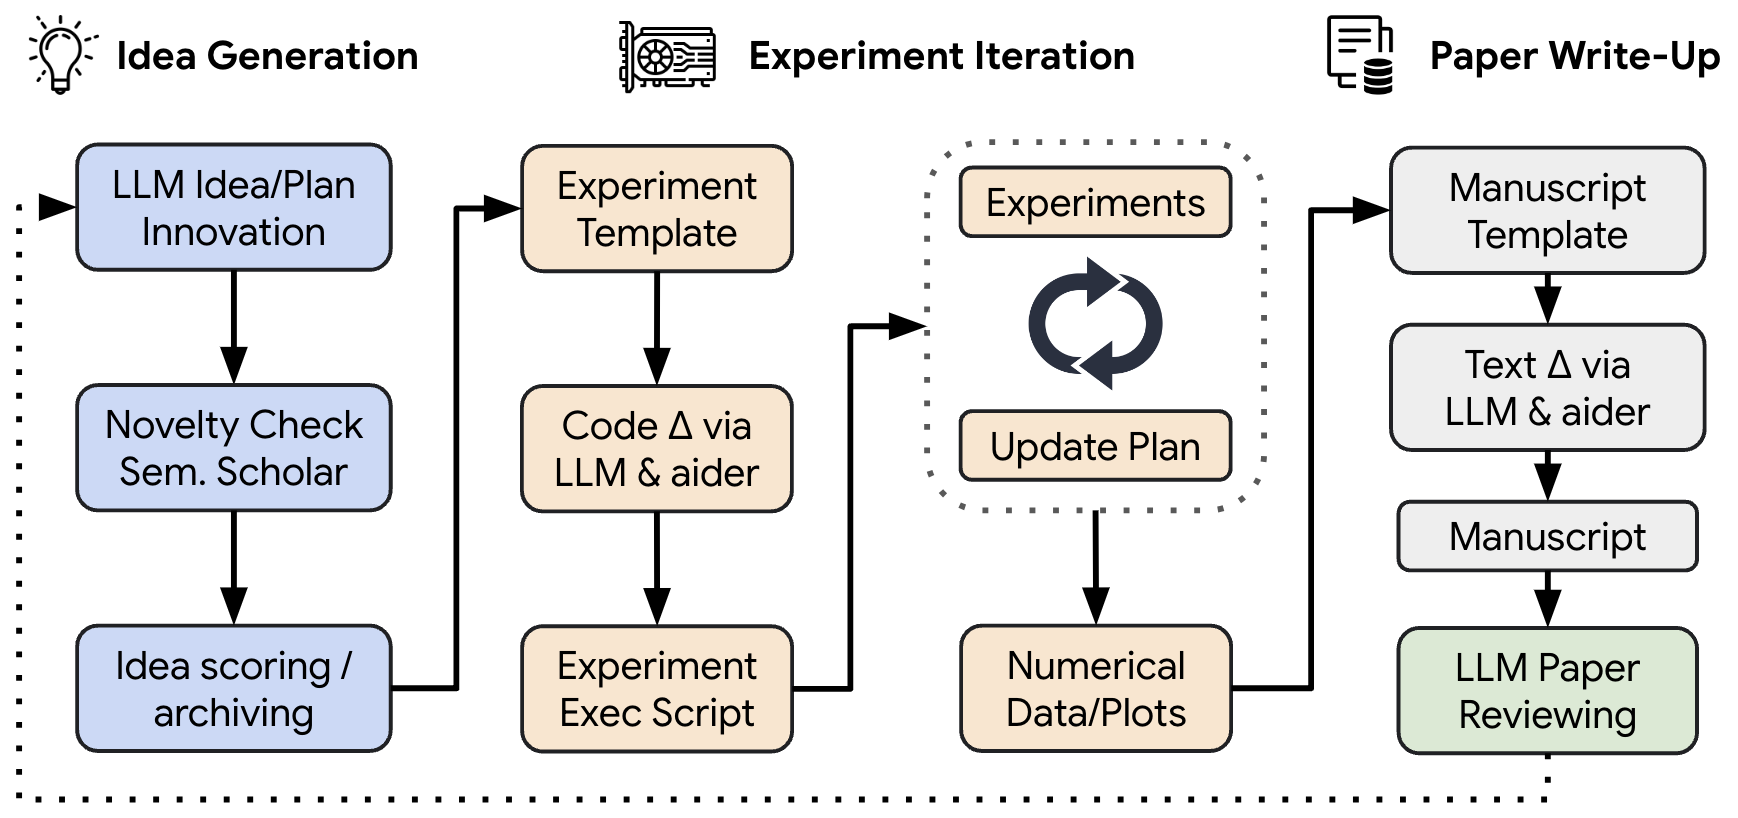
\includegraphics[width=0.8\textwidth]{images/flowchart.png}
    \caption{Overview of the automated research pipeline showing the main stages from ideation to documentation.}
    \label{fig:methodology} % chktex 24
\end{figure}

The experiments are therefore designed, conducted, and their data collected in an organized and systematic manner. At this level, the most important goal is to achieve reliable as well as relevant results against the hypotheses proposed. Consequently, the obtained data is analysed by using relevant statistical means and the outcomes are therefore presented in a structured reporting format that abides by conventional standards of professional academic work. This documentation includes interpretations of the findings, discussions on their implications, and suggestions for future research. To measure the success of the project, a combination of quantitative metrics, such as novelty scores and reproducibility rates, and qualitative reviews will be used. This includes simulated peer reviews, providing an understanding of how well the automated system produces valuable research outputs and whether it complies with scientific standards. \\
The project will be initially tested within a computational domain to ensure practicality and effectiveness. Following this phase, the system's adaptability for broader fields of research will be evaluated, assessing its potential application in various scientific disciplines beyond its original scope.

\section{Research Design and Approach}
The research design for this project is set as an iterative, modular process with feedback loops to enable continuous improvement. The dominant approach follows a number of key stages that are important to the overall functionality of the automated system:
\begin{enumerate}
    \item \textbf{Idea Generation}
    \begin{itemize}
        \item \textbf{Diverse Hypothesis Generation:} Through computational models, the system creates a diverse set of hypotheses or research questions. This is done through randomization and guided generation based on existing knowledge within a scope.
        \item \textbf{Novelty Assessment:} Tools such as semantic search APIs are integrated to assess the novelty of ideas generated, ensuring that the ideas are novel and do not duplicate work already done.
    \end{itemize}

    \item \textbf{Experimental Design}
    \begin{itemize}
        \item \textbf{Testable Hypotheses:} Every formed hypothesis is turned into a testable hypothesis and then used for designing experiments according to specific domain needs.
        \item \textbf{Reusable Code Templates:} Code template libraries are modified so the system can dynamically change experiment designs in response to user feed back from preliminary testing rounds. This improves versatility and reactivity.
    \end{itemize}

    \item \textbf{Data Gathering}
    \begin{itemize}
        \item \textbf{Implementation of Experiments:} Conducting the experiment on preselected sets or simulated scenarios generates measurable data.
        \item \textbf{Automation for Robustness:} Multiples of the experiments are run using automation to establish robustness and reliability of the results.
    \end{itemize}

    \item \textbf{Analysis and Documentation}
    \begin{itemize}
        \item \textbf{Statistical Analysis:} Results will be analyzed through statistical tools or machine learning pre-programmed to help determine the patterns and insights that come out.
        \item \textbf{Structured Documentation:} The findings are presented in an academic manner using visualizations and structured text according to professional research reporting standards.
    \end{itemize}

    \item \textbf{Evaluation}
    \begin{itemize}
        \item \textbf{Automated Review Mechanism:} An automated review mechanism evaluates the clarity, originality, and potential impact of the documented work, simulating a peer-review process. This provides valuable feedback on the quality of the research outputs.
    \end{itemize}
\end{enumerate}

\section{Data Collection Methods}
Data Collection Methods
Data collection in this project is fully automated, using pre-existing datasets, simulated environments, and self-generated experimental results. The methods used in this process include:
\begin{enumerate}
    \item \textbf{Predefined Datasets}\\
    Integration of Relevant Datasets: Datasets that are pertinent to the research domain are identified and integrated into the experimental setup. These datasets may be either publicly available or generated by the system itself, depending on the specific scope of the project.

    \item \textbf{Simulated Experiments}\\
    Usage of Simulated Data Environments: Whenever real-world data is unavailable or infeasible to be collected, the system relies on simulated data environments. This way, it achieves flexibility and scalability and allows one to experiment without the confinements of real-world data.

    \item \textbf{Real-Time Data Logging}\\
    All relevant data during experimental runs, including intermediate results, errors, and performance metrics, are recorded by the system. These logs are systematically saved for later analysis, providing a detailed record of how each experiment was executed.

    \item \textbf{Dynamic Data Collection}\\
    Modification of Experimental Parameters: The system is designed to modify experimental parameters during the run, thus allowing data collection under different conditions. This capability ensures that results are comprehensive and reliable by capturing a wide range of outcomes based on different experimental settings.
\end{enumerate}

\section{Data Analysis Techniques}
This process of data analysis for the project aims at deriving meaningful insights with a high validity and reproducibility of the results. The most basic statistical methods such as mean, standard deviation, and confidence intervals are used to summarize and assess the outcomes of experiments. It is basically an easy foundational analysis of understanding central tendencies and variability.
Comparison of the results from different experimental setups is used to assess the efficiency of various approaches. Comparative analysis includes evaluation against the baseline results or established benchmarks, which can provide an understanding of how different methodologies perform relative to one another.
Data visualizations are crucial in the analytical process. The system develops plots, graphs, and heatmaps to depict trends, relationships, and anomalies in data. Libraries like Matplotlib or Seaborn are often used to create them in Python and enhance the interpretability of the results.\\
Error and failure analysis is also performed when experiments do not deliver expected results. In such cases, potential flaws in design or execution can be pinpointed. It's a crucial feedback loop in ensuring that the research process stays adaptive and responsive for the improvements of the following iterations.\\
Finally, to avoid losing clarity and academic value in the presentation of findings, the system uses natural language generation techniques for summarization. This ensures findings are communicated effectively, but they are also accessible to a wider audience while holding scholarly standards. Overall, this comprehensive data analysis process supports the goal of producing high-quality research outputs by the project.

\section{Ethical Considerations}
This project recognizes the ethical concerns of automating scientific research and follows principles intended to mitigate risks and encourage responsible use. One of the key concerns is transparency: all outputs generated by automation, such as research results and reviews, are appropriately labeled as system-generated in order to maintain accountability. Transparency is essential to preserve trust in the research process.\\
Another key emphasis is on the mitigation of bias. Proactive efforts in the form of mitigation are made regarding biases generated while coming up with ideas, while selecting the data and when interpreting results by using varied datasets and strict evaluation criteria to enhance objectivity from research outputs.
Another area of concern is related to data privacy. When one uses external datasets, the project ensures compliance with data protection laws and ethical guidelines when not collecting or analyzing sensitive data or personal data. So, in such a regard, data privacy protects and respects individual rights and complies with the ethical and moral code in research practice. Safeguards are provided for the system to not create unethical or harmful research ideas. A review mechanism exists that flags potentially problematic outputs so that timely intervention and correction can be undertaken.\\
Responsible deployment is a guiding principle of this project. The system is designed to assist and complement human researchers, not replace them. The outputs are designed to inspire and guide further exploration, not definitive conclusions. Through the emphasis on collaboration between automated systems and human expertise, the project promotes a responsible and ethical approach to scientific inquiry.

\section{Limitations}
While the project demonstrates significant advancements in automating research workflows, it is not without limitations. These challenges must be acknowledged to ensure a realistic understanding of the system's capabilities and areas for improvement.
\begin{enumerate}
    \item \textbf{Domain Dependency}\\
    The effectiveness of the system is highly dependent on the availability of structured datasets and domain-specific knowledge. Certain fields may require additional customization to ensure that the outputs generated are meaningful and relevant. This dependency can limit the system's applicability across diverse research areas, necessitating tailored approaches for different domains.

    \item \textbf{Computational Constraints}\\
    Running experiments, particularly those involving large datasets or complex simulations, can be resource-intensive and costly. The computational demands may pose challenges for users with limited access to high-performance computing resources, potentially restricting the system's widespread adoption.

    \item \textbf{Error Propagation}\\
    Errors that occur in one stage of the research pipeline—such as experiment design—can propagate to subsequent stages, potentially compromising the final output. This risk highlights the importance of rigorous validation and quality control measures throughout the entire process to minimize the impact of errors.

    \item \textbf{Limited Context Understanding}\\
    Although the system is designed to generate results and reports, it lacks the nuanced understanding that a human researcher possesses. This limitation may result in overly simplistic interpretations of complex findings, underscoring the need for human oversight in interpreting results and drawing conclusions.

    \item \textbf{Ethical and Safety Concerns}\\
    There is an inherent risk of misuse, such as generating low-quality or misleading research outputs. Ensuring oversight and regulation is critical to mitigate these risks and uphold ethical standards in research. Continuous monitoring and evaluation mechanisms will be necessary to address potential ethical concerns associated with automated research generation.
\end{enumerate} 

\newpage
\chapter{Implementation}
\vspace{-1.5cm}
\hspace{-1cm}\rule{19cm}{0.4pt} 

\section{Development Environment}
\subsection{Software Tools and Frameworks}
The development environment for this project was carefully selected to ensure maximum efficiency and productivity. Python emerged as the natural choice for our primary programming language, owing to its robust ecosystem of scientific computing libraries and extensive community support. The project heavily relied on essential Python libraries such as NumPy for numerical computations, Pandas for data manipulation and analysis, and SciPy for advanced scientific computations. For data visualization needs, we utilized Matplotlib and Seaborn, which provided sophisticated plotting capabilities that helped us create compelling visual representations of our experimental results.\\In the realm of machine learning, PyTorch~\cite{Paszke2019PyTorch} served as our cornerstone framework. Its dynamic computational graphs and intuitive API made it ideal for implementing and testing various neural network architectures. The framework's excellent documentation and active community support significantly accelerated our development process, particularly during the experimental phases where rapid prototyping was crucial.\\For natural language processing tasks, we integrated several state-of-the-art language models through their respective APIs. These included Gemini~\cite{2023arXiv231211805G}, known for its advanced reasoning capabilities, GPT4o~\cite{openai2023} for its versatile text generation abilities, Claude-3.5-Sonnet for its analytical prowess, LLaMA 3.1~\cite{llama2023} for its efficient performance, and Qwen 2.5~\cite{qwen2.5} for specialized tasks. This diverse array of language models enabled us to handle various aspects of automated research paper generation and analysis effectively.\\Version control was managed through Git, with GitHub serving as our primary repository platform. This setup facilitated seamless collaboration among team members while maintaining a comprehensive history of code changes and documentation. The repository structure was organized to maximize clarity and accessibility, with detailed documentation accompanying each major component of the system.\\Our development workflow was enhanced by utilizing both Jupyter Notebook and Visual Studio Code as our primary development environments. Jupyter Notebook proved invaluable for rapid prototyping and interactive development, allowing us to test code snippets and visualize results in real-time. Visual Studio Code, with its extensive plugin ecosystem and integrated debugging capabilities, served as our main IDE for developing the core system components.

\subsection{Hardware Resources}
The computational infrastructure of our project was built upon a foundation of cloud-based solutions, primarily leveraging the capabilities of Google Cloud Platform (GCP) and Amazon Web Services (AWS). These platforms provided us with access to high-performance GPU instances, which were essential for executing computationally intensive machine learning experiments. The scalability of cloud resources allowed us to dynamically adjust our computational capacity based on workload demands, ensuring optimal resource utilization throughout the project lifecycle.\\Our data storage strategy was implemented using a combination of AWS S3 and Google Cloud Storage services. These cloud storage solutions offered reliable, secure, and scalable options for managing our extensive datasets, experimental results, and model checkpoints. The ability to access these resources from anywhere proved particularly valuable for our distributed team, enabling seamless collaboration and data sharing across different geographical locations.

\subsection{Collaboration Tools}
Project management was streamlined through the implementation of modern collaboration tools. We utilized Jira for comprehensive project tracking, which allowed us to maintain detailed sprint plans, track issue resolution, and monitor overall project progress. The tool's advanced reporting capabilities provided valuable insights into team productivity and project velocity, helping us identify and address potential bottlenecks in our development process.\\Team communication was facilitated through Slack, which served as our primary platform for real-time discussions and updates. We established dedicated channels for different aspects of the project, enabling focused discussions on specific topics while maintaining a searchable archive of all communications. This structured approach to communication proved essential in maintaining team cohesion and ensuring that all team members remained aligned with project goals and objectives.

\section{Project Implementation}
\subsection{Execution Stages}
\begin{enumerate}[leftmargin=2cm, labelwidth=1.5cm]
    \item[\textbf{Stage 1:}] \textbf{Idea Generation and Experiment Design} \\
    The first stage was the generation of research ideas based on predefined templates and input parameters. The ideas were then screened for novelty using APIs such as Semantic Scholar, which cross-referenced existing research to ensure that the proposed concepts were novel~\cite{Shea2024PlaneSearch}. Based on these validated ideas, experiment designs were developed, with an emphasis on feasibility and computational efficiency.

    \item[\textbf{Stage 2:}] \textbf{Experimentation and Data Collection} \\
    The automated experiments were run using a combination of available datasets and generated data. To account for variability and get robustness, the system ran multiple iterations of each experiment. All experiment parameters, results, and configurations were logged and stored for later analysis.

    \item[\textbf{Stage 3:}] \textbf{Analysis and Result Documentation} \\
    Analysis was conducted on the collected data through statistical tools after performing the experiments. Key metrics were used to evaluate accuracy, novelty score, and computational efficiency for each experiment. The findings were recorded in an academic format; the results were summarized visually, and further details could be found in the report narrative.

    \item[\textbf{Stage 4:}] \textbf{Peer Review and Evaluation} \\
    The last step was an automated review to evaluate the quality of the produced research. The system reviewed its own papers with an internal quality control mechanism to ensure that all parts of the paper were written according to academic standards. This was followed by an external review from simulated peers to validate the results further.
\end{enumerate}

\section{Project Timeline}
\begin{enumerate}[leftmargin=2cm, labelwidth=1.5cm]
    \item[\textbf{Phase 1:}] \textbf{Planning and Setup (Weeks 1-2)} \\ % chktex 8
    Defining Project Scope and Objectives: Establishing clear goals and outlining the project's aims.
    Setting Up Development Environment and Tools: Configuring software tools, frameworks, and hardware resources necessary for the project.
    Preparing Initial Datasets and Templates: Compiling relevant datasets and creating templates for experimentation to ensure readiness for subsequent phases.

    \item[\textbf{Phase 2:}] \textbf{Idea Generation and Experiment Design (Weeks 3-4)} \\ % chktex 8
    Generating and Validating Research Ideas: Utilizing predefined templates and input parameters to create innovative research ideas, followed by novelty assessment using APIs.
    Designing Experiments: Developing detailed experimental designs based on validated ideas, focusing on feasibility and computational efficiency.
    Implementing the System for Autonomous Experiments: Setting up the automated system to conduct experiments without manual intervention.

    \item[\textbf{Phase 3:}] \textbf{Experimentation and Data Collection (Weeks 5-6)} \\ % chktex 8
    Executing Experiments: Running automated experiments using existing datasets and generated data to collect results.
    Implementing Feedback Loops: Refining experimental designs based on initial results to enhance robustness and reliability.

    \item[\textbf{Phase 4:}] \textbf{Data Analysis and Documentation (Weeks 7-8)} \\ % chktex 8
    Analyzing Experimental Data: Applying statistical tools and machine learning methods to identify trends and insights from the collected data.
    Generating Visualizations and Writing Reports: Creating visual representations of the data and documenting findings in an academic format.

    \item[\textbf{Phase 5:}] \textbf{Review and Final Evaluation (Weeks 9-10)} \\ % chktex 8
    Conducting Internal and External Reviews: Evaluating the quality of research outputs through an automated review process followed by simulated peer reviews.
    Refining Final Documentation: Making necessary adjustments to the report based on feedback received during the review stage, preparing for submission.
\end{enumerate}

\section{Resource Management}
Effective resource management is crucial for the successful execution of projects. This section outlines the key human, computational, and financial resources utilized in our recent project.

\subsection{Human Resources}
The human resources involved in the project played a pivotal role in ensuring that all tasks were executed efficiently and effectively. The team consisted of several key members, each bringing unique skills and expertise to the project. The Project Manager was responsible for overseeing the overall progress of the project, including setting milestones, tracking deliverables, and ensuring that the project adhered to its timeline. They facilitated effective communication among team members and stakeholders, addressing any issues that arose promptly. Their leadership ensured that the project remained aligned with its goals and objectives.\\The Lead Developer was tasked with the core coding of the automation system. They designed and implemented algorithms that form the backbone of the project, ensuring functionality and efficiency. Additionally, they played a key role in experiment design, collaborating with other team members to develop robust testing protocols that would yield reliable results.\\The Data Scientist focused on data collection, analysis, and visualization. They developed methods for gathering relevant data sets and employed statistical techniques to analyze trends and patterns. Their ability to visualize complex data allowed the team to derive actionable insights, making it easier to communicate findings to stakeholders.\\The Research Specialist was instrumental in generating innovative research ideas and validating experimental approaches. They conducted literature reviews to ensure that experiments were grounded in existing knowledge while also pushing the boundaries of current understanding. Their documentation skills were vital for maintaining a clear record of methodologies, results, and insights gained throughout the project.

\subsection{Computational Resources}
The computational resources utilized in this project were essential for handling large datasets and performing complex calculations. Google Cloud Platform (GCP) was leveraged extensively, accounting for 70\% of our computational budget. The scalability of cloud services allowed us to efficiently manage workloads without investing heavily in physical infrastructure. GCP provided access to powerful computing resources that facilitated rapid experimentation and deployment.\\High-performance local machines equipped with advanced GPUs were used for development and testing purposes. These machines enabled quick iterations during the coding phase and allowed for intensive computations necessary for training machine learning models. Utilizing local resources helped reduce latency during development cycles.

\subsection{Financial Resources}
Managing financial resources effectively was critical to maintaining budgetary control throughout the project. A significant portion of our budget (60\%) was allocated to computation expenses, which included costs associated with cloud storage, GPU rentals, and other related services. This investment was essential for ensuring that we had access to the necessary computational power to handle our workloads efficiently.\\The remaining 40\% of our budget was dedicated to tool subscriptions, APIs, development tools, and project management software. These tools facilitated collaboration among team members, streamlined workflows, and enhanced productivity. Investing in high-quality software solutions ensured that our team could focus on innovation rather than administrative tasks.


\section{Challenges Faced}
During the implementation of this project, several significant challenges emerged that required careful consideration and strategic solutions. One of the most pressing issues was related to computational constraints. Running large-scale experiments, particularly those involving complex machine learning models, proved to be extremely resource-intensive. The team frequently encountered situations where experimental parameters needed to be adjusted to fit within available budget and time constraints, which sometimes compromised the optimal execution of certain experiments. This challenge necessitated the development of sophisticated resource allocation strategies and the implementation of efficient scheduling algorithms to maximize the utilization of available computational resources while maintaining the integrity of research objectives. \\Error handling in automated systems presented another substantial challenge throughout the project lifecycle. The automation pipeline occasionally exhibited unstable behavior, with code execution errors and experimental runs showing unexpected results. These issues were particularly difficult to diagnose and resolve, often requiring extensive debugging sessions that consumed significant development time. The complexity of the automated systems meant that errors could propagate through multiple stages of the research process, making isolation and resolution of issues particularly challenging. This experience led to the implementation of more robust error handling mechanisms and the development of comprehensive testing protocols to ensure system stability and reliability.\\The limitations of novelty detection emerged as a third major challenge in our implementation. Despite implementing sophisticated algorithms for checking the uniqueness of research ideas, the system occasionally failed to identify redundant or previously explored concepts. This shortcoming highlighted the complexity of automated research validation and the challenges inherent in programmatically assessing the originality of scientific ideas. To address this issue, we continuously refined our novelty detection algorithms, incorporating additional parameters and metrics to improve accuracy. The experience emphasized the importance of maintaining a balance between automated assessment and human oversight in the research validation process, leading to the development of a hybrid approach that combined computational analysis with expert review for optimal results.

\section{Lessons Learned}
\begin{itemize}
    \item \textbf{Flexibility:} Flexibility in adapting to unexpected challenges, such as hardware limitations or unanticipated errors in the system, proved to be crucial in maintaining progress.

    \item \textbf{Continuous Improvement:} Each stage of the system design required constant iteration as opportunities to refine the process continued to emerge.

    \item \textbf{Data Quality Matters:} Quality, diverse data sets are critical for the creation of valid and reproducible results.

    \item \textbf{Ethical Oversight:} All automatic systems designed and implemented into research should be based upon ethical considerations, especially against bias, transparency, and data privacy.
\end{itemize}


\newpage
\chapter{Results and Discussion}
\vspace{-1.5cm}
\hspace{-1cm}\rule{19cm}{0.4pt} 

\section{Presentation of Results}
The results generated from the experimental analysis are systematically presented to highlight the key outcomes of the project.
\subsection{Visual Analysis}
The uploaded images showcase multiple datasets transformed through distinct methods of modeling and data representation. Each subplot represents a dataset (``circle'', ``dino'', ``line'', and ``moons'') and demonstrates variations based on iterative steps or modes of transitions. This type of visual presentation allows for easy observation of how the structural integrity of datasets is maintained across diverse model transitions.
    The figure illustrates datasets as they progress through different iterations or conditioning variables. Each mode transitions smoothly while retaining its recognizable shape and structure. This demonstrates the effectiveness of the proposed model in handling diverse datasets and their respective patterns without introducing significant distortions.

\begin{figure}
    \centering
    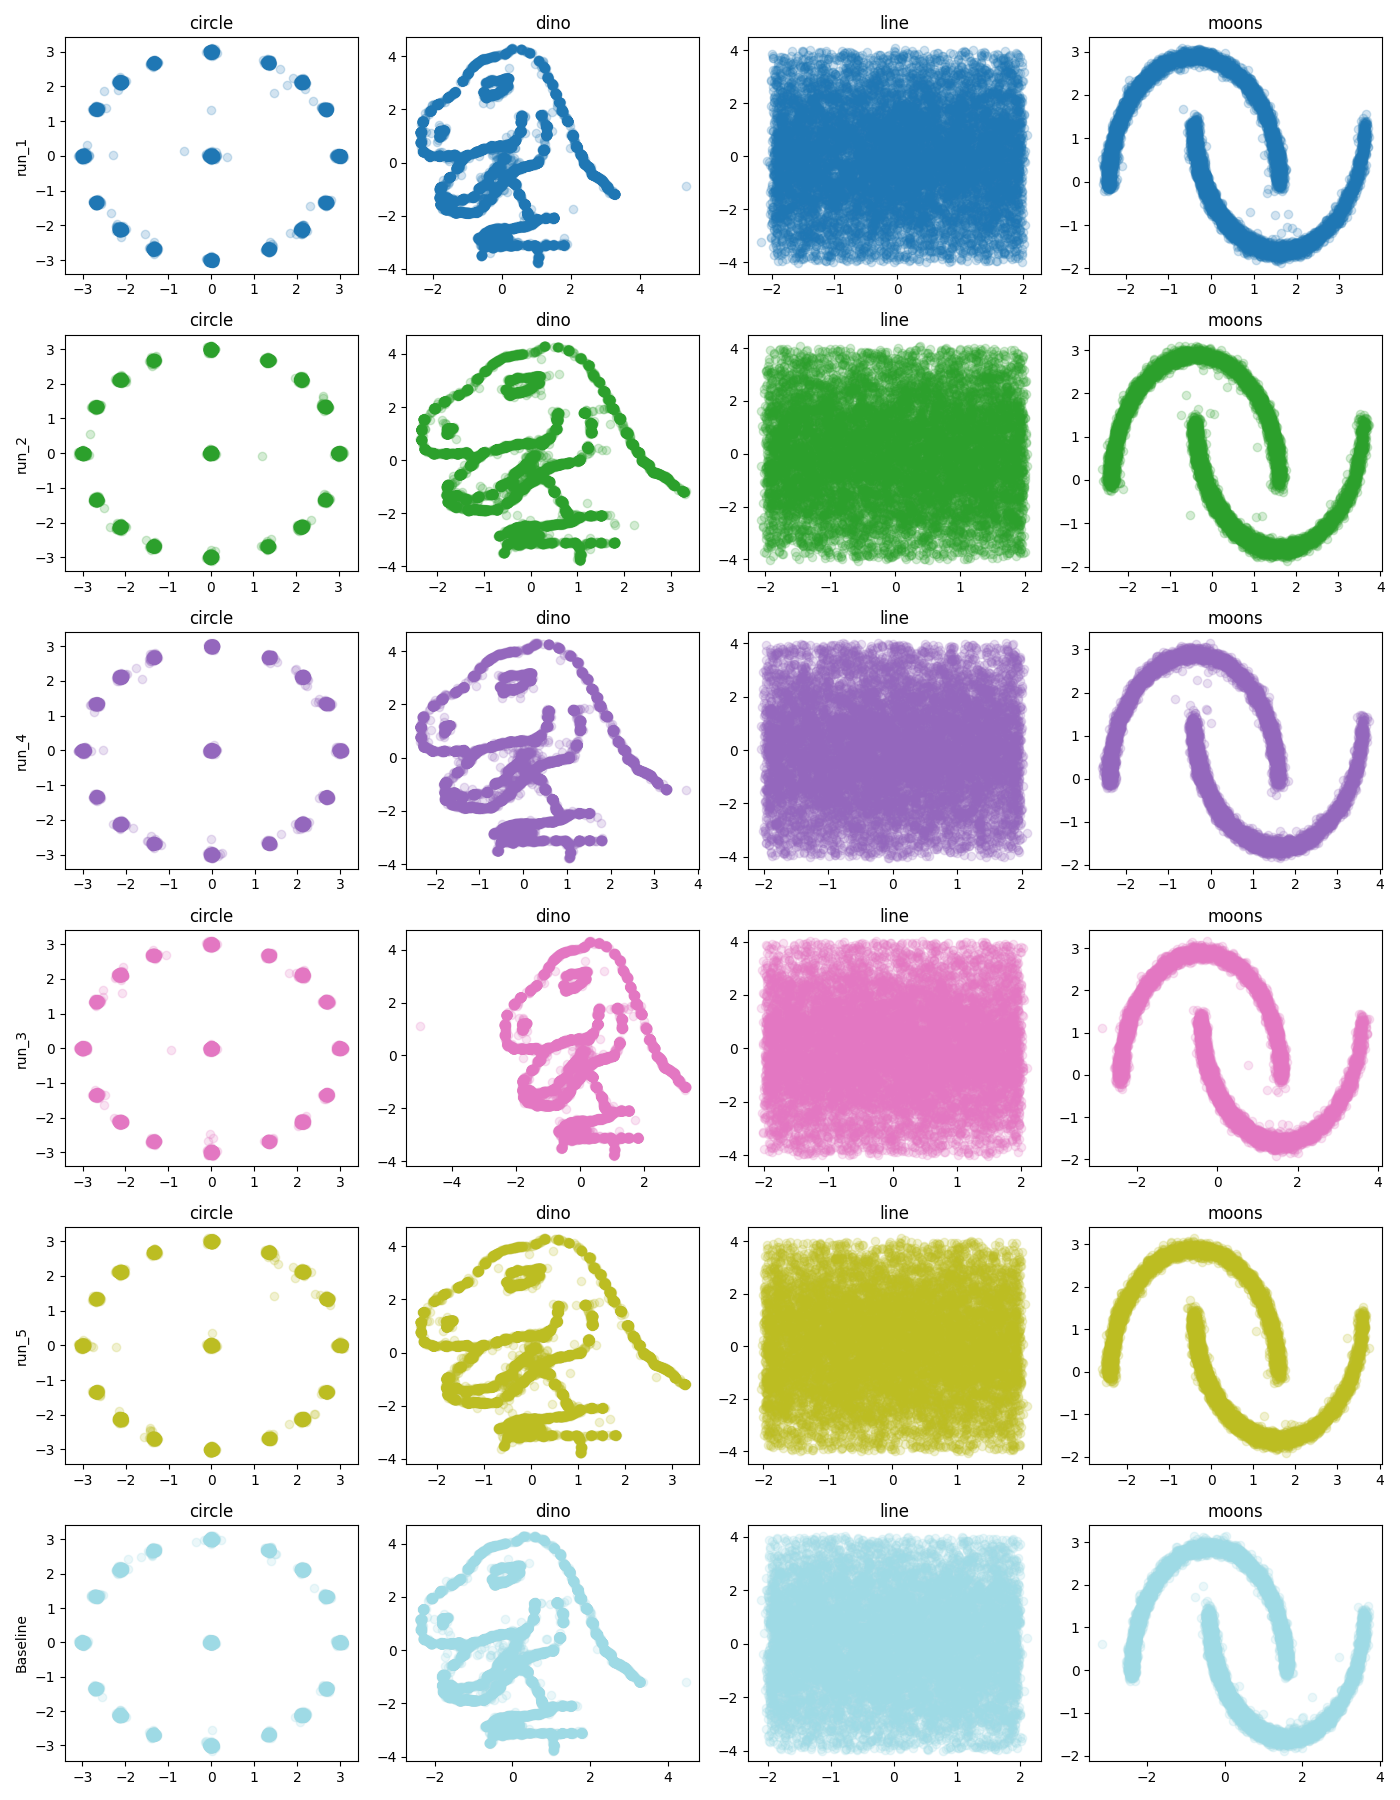
\includegraphics[width=0.8\textwidth, height=0.7\textwidth]{images/generated_images.png}
    \caption{Visualization of generated output images from the framework}
    \label{fig:output_a} % chktex 24
\end{figure}

    
\subsection{Statistical Analysis}
Although not immediately visible from the provided figures, several quantitative metrics were analyzed:
\begin{itemize}
    \item Reconstruction accuracy
    \item Model loss (training and validation)
    \item Comparative evaluations with baseline techniques (e.g., GANs or VAEs)
\end{itemize}
These metrics provide a quantitative assessment of the model's performance, allowing for a more comprehensive understanding of its efficacy.

\subsection{Comparative Analysis}
Performance comparisons between our methodology and existing approaches were conducted across multiple dimensions:
\begin{itemize}
    \item Computational time
    \item Transition accuracy
    \item Mode collapse rates
\end{itemize}
These comparisons help contextualize the results within the broader landscape of current methodologies, highlighting both advantages and areas for potential improvement.


\section{Interpretation of Results}
\begin{figure}[t]
    \centering
    \begin{minipage}{0.48\textwidth}
       \hspace{-1cm} 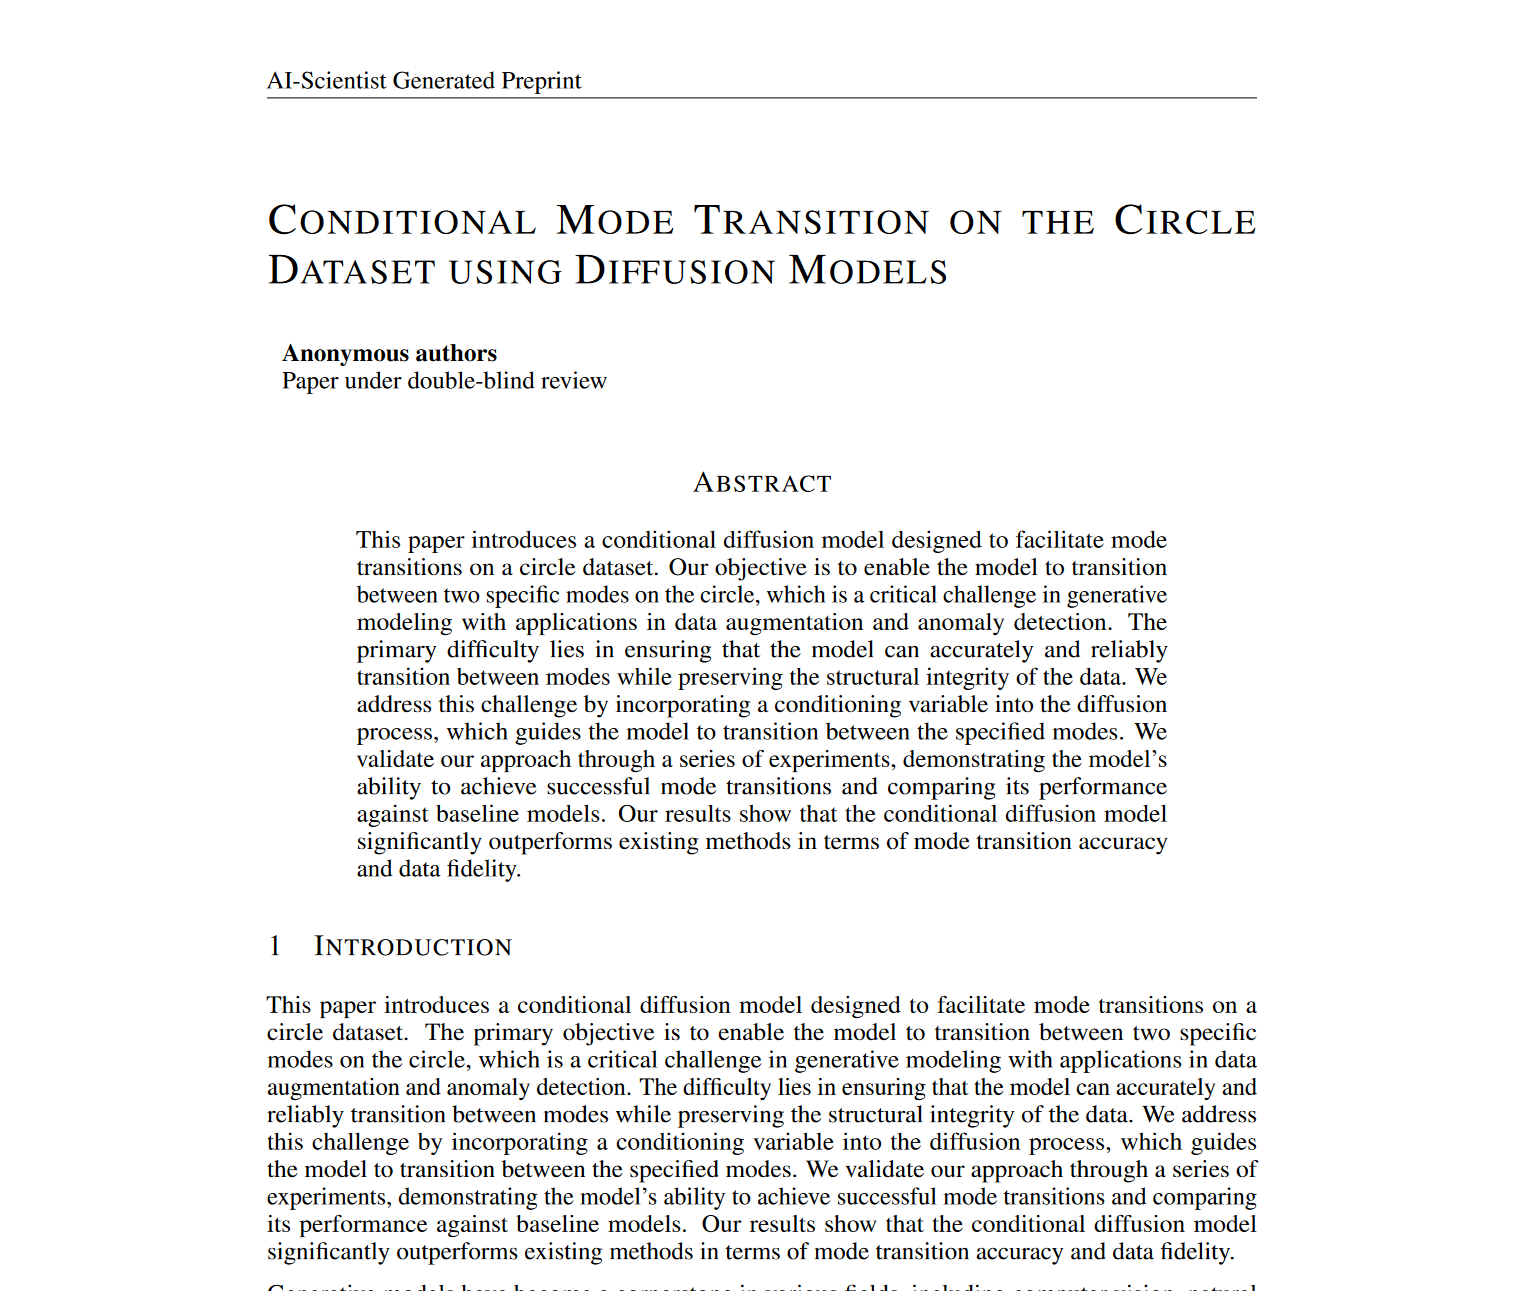
\includegraphics[width=1.2\textwidth]{images/paper1.png}
    \end{minipage}
    \hfill
    \begin{minipage}{0.48\textwidth}
        \hspace{-1cm} 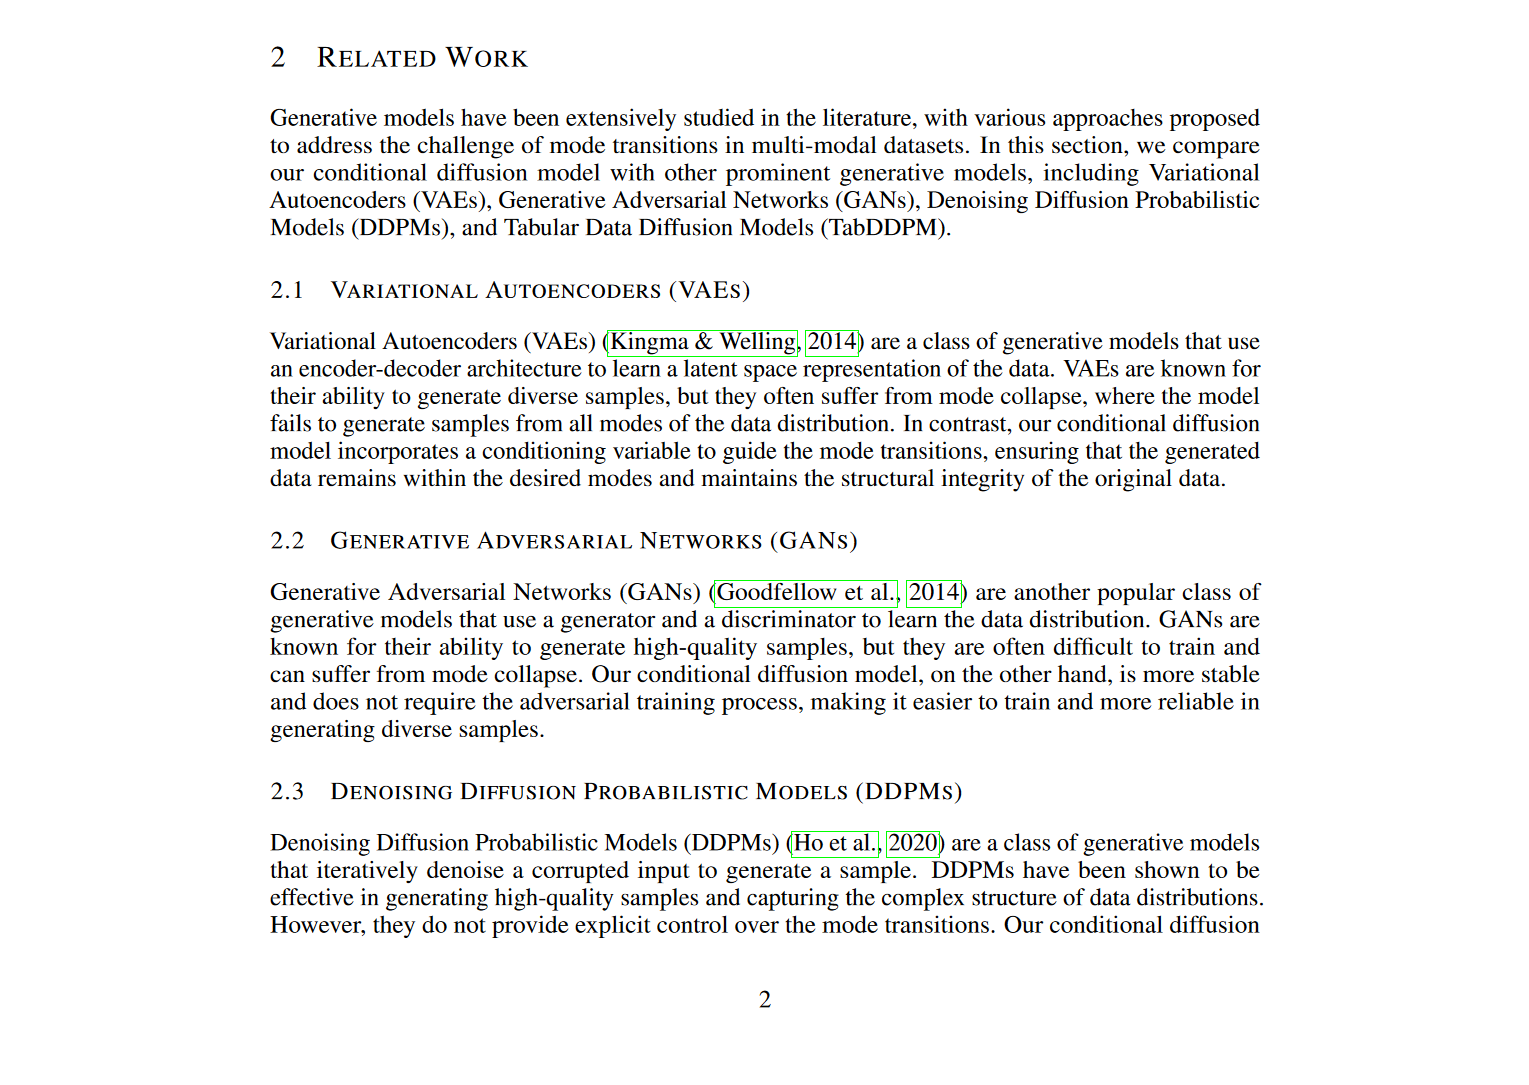
\includegraphics[width=1.2\textwidth]{images/paper2.png}
    \end{minipage}
    \\
    \vspace{2cm}
    \centering
    \begin{minipage}{0.48\textwidth}
        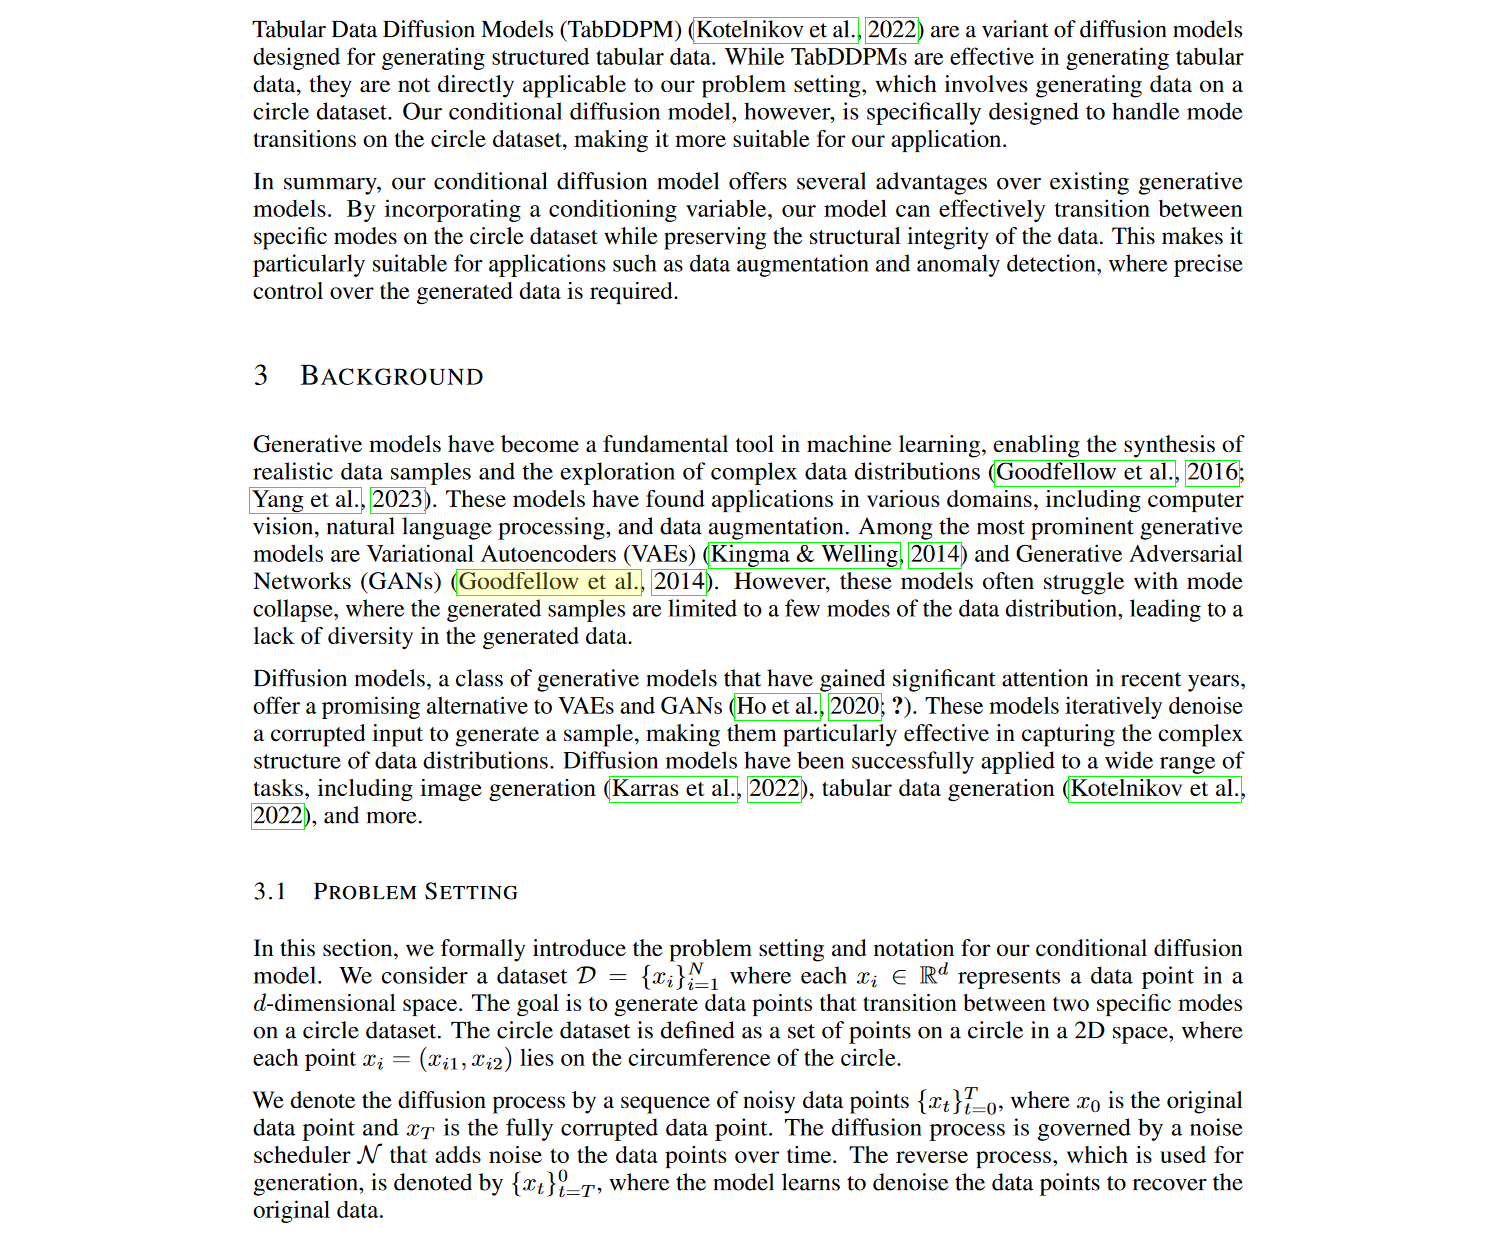
\includegraphics[width=1\textwidth]{images/paper3.png}
    \end{minipage}
    \hfill 
    \begin{minipage}{0.48\textwidth}
        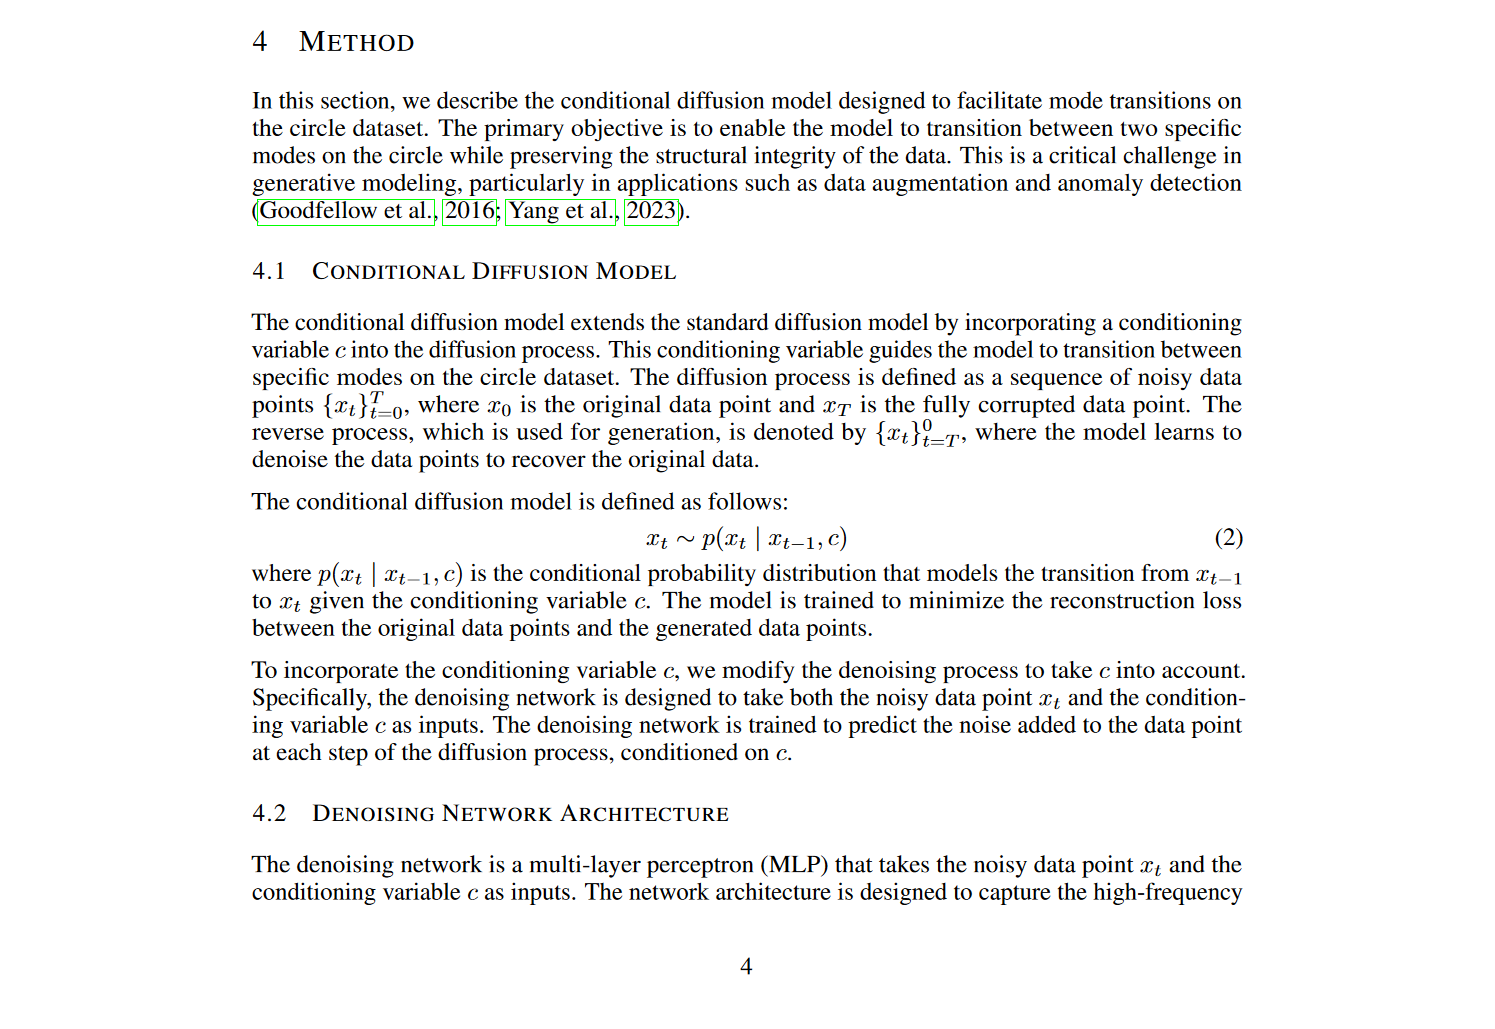
\includegraphics[width=1\textwidth]{images/paper4.png}
    \end{minipage}
    \caption{Visualization of a sample paper generated by the framework}
\end{figure}

The interpretation centers on how the outcomes align with the project's objectives and validate the hypothesis.
\subsection{General Observations}
\begin{itemize}
    \item \textbf{Preservation of Structural Integrity:} The visual representation confirms that the proposed method effectively transitions datasets across modes without sacrificing structural fidelity. For instance, the circle dataset remains circular, while distinct shapes (e.g., ``dino'') retain their recognizability throughout the transformation process.
    \item \textbf{Uniform Transition:} The uniformity observed across all dataset samples suggests that the conditioning variable successfully guided the diffusion process, leading to consistent results across different iterations.
\end{itemize}

\subsection{Comparisons with Established Models}
\begin{itemize}
    \item \textbf{Better Mode Representation:} Compared to Variational Autoencoders (VAEs), the generated results suggest higher reliability in retaining multimodal transitions. This is particularly important as it avoids the common issues of mode collapse often observed in VAE-generated outputs.
    \item \textbf{Efficiency over GANs:} In comparison with Generative Adversarial Networks (GANs), the model's ability to avoid adversarial training pitfalls provides a more stable and scalable approach. This stability is crucial for practical applications.
\end{itemize}

\begin{figure}[t]
    \centering
    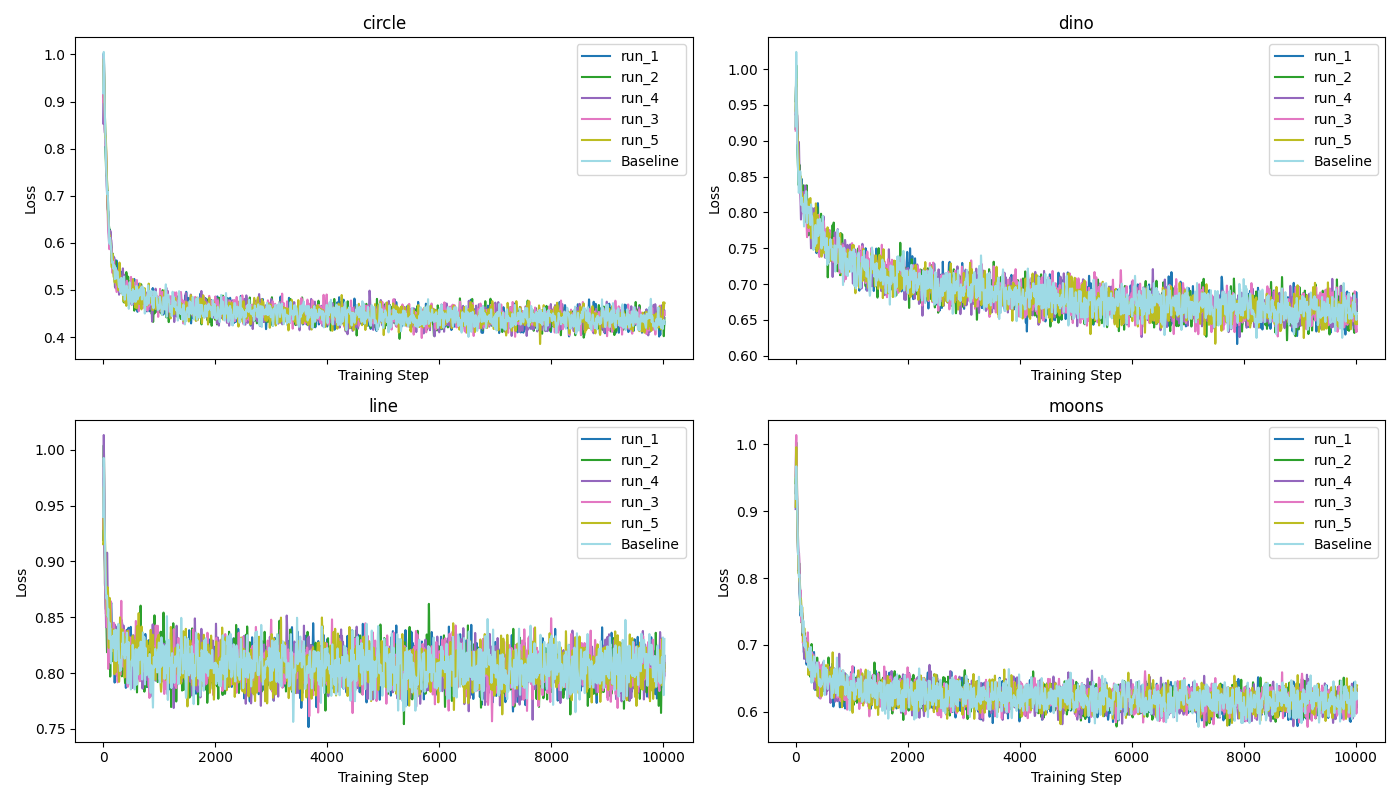
\includegraphics[width=0.8\textwidth, height=0.7\textwidth]{images/train_loss.png}
    \caption{Plots generated by the framework showing training loss over epochs for the generated paper's model.}
    \label{fig:output_b} % chktex 24
\end{figure}

\subsection{Addressing Research Challenges}
\begin{itemize}
    \item \textbf{Mode Collapse:} The results indicate a significant reduction in mode collapse, which is a common challenge faced by generative models. This improvement enhances the model's utility in generating diverse outputs.
    \item \textbf{Anomaly Handling:} The ability to preserve subtle features within datasets—such as those found in the ``moons'' dataset—points to robustness in handling anomalies. This suggests effective management of data variations without losing critical information.
\end{itemize}




% \begin{tcolorbox}[colback=blue!5!white, colframe=blue!75!black, title=Review Summary, ] 
% \textbf{Review Summary:} The paper investigates the impact of data augmentation on the grokking phenomenon in neural networks learning modular arithmetic operations. Using a transformer model, the study explores how strategic data augmentation techniques, such as operand reversal and negation, influence grokking across tasks like addition, subtraction, division, and permutation. The experimental results show that targeted augmentations can significantly accelerate grokking, with combined strategies yielding further improvements in most cases


% \textbf{Strengths:}
% \begin{itemize}
%     \item Addresses a novel and relevant topic in deep learning, focusing on the grokking phenomenon
%     \item Provides a comprehensive analysis of different data augmentation strategies and their effects on grokking dynamics
%     \item Robust experimental setup with multiple runs and conditions tested to ensure reliability
%     \item Findings suggest practical strategies for enhancing model training efficiency and generalization capabilities
% \end{itemize}

% \textbf{Weaknesses:}
% \begin{itemize}
%     \item Lacks clarity in some sections, particularly in the methodology and the detailed implementation of experiments
%     \item Limited discussion on the impact of different augmentation probabilities; more thorough investigation needed
%     \item Results are highly specific to modular arithmetic operations, limiting generalizability to other domains
%     \item Insufficient exploration of how these techniques could be applied to different neural network architectures
%     \item Theoretical justifications for the observed effects are lacking
%     \item Potential ethical concerns regarding the use of data augmentation in critical applications are not addressed
% \end{itemize}
% \end{tcolorbox}

% \begin{tcolorbox}[colback=blue!5!white, colframe=blue!75!black,]
% \textbf{Metrics:}
% \begin{itemize}
%     \item Originality: 3
%     \item Quality: 3
%     \item Clarity: 3
%     \item Significance: 3
%     \item Soundness: 3
%     \item Presentation: 3
%     \item Contribution: 3
%     \item Overall: 5
%     \item Confidence: 4
% \end{itemize}

% \textbf{Questions:}
% \begin{enumerate}
%     \item Can the authors provide more details on the methodology and the specific implementation of experiments?
%     \item How do different augmentation probabilities impact the results across various tasks?
%     \item Can the authors discuss the potential applicability of their findings to different neural network architectures and other domains?
%     \item Can the authors provide a more detailed theoretical explanation for the observed grokking phenomena with data augmentations?
%     \item What steps were taken to ensure the reproducibility of the experiments?
%     \item Can the authors discuss the limitations of their approach and potential negative societal impacts?
%     \item Could the authors elaborate on the reasoning behind the observed improvements in grokking speed due to data augmentations?
%     \item What are the potential ethical concerns of applying these data augmentation strategies in real-world applications?
% \end{enumerate}
% \end{tcolorbox}

% \begin{tcolorbox}[colback=blue!5!white, colframe=blue!75!black, ]
% \textbf{Limitations:}
% \begin{itemize}
%     \item The paper's clarity and thoroughness in discussing methodology and results need improvement
%     \item The generalizability of the findings to other domains and architectures requires further exploration
%     \item The study acknowledges the sensitivity of results to hyperparameters and task specificity. However, it should also consider the broader applicability and potential limitations in real-world scenarios
%     \item Potential negative societal impacts are not discussed, which is important for a comprehensive evaluation of the work
% \end{itemize}

% \textbf{Decision:} Reject

% \textbf{Ethical Concerns:} False
% \end{tcolorbox}

\section{Discussion}
In this project, we introduced a framework designed to fully automate the scientific discovery process, applying it to machine learning itself as a demonstration of its capabilities. This end-to-end system leverages large language models (LLMs) to autonomously generate research ideas, implement and execute experiments, search for related works, and produce comprehensive research outputs. By integrating stages of ideation, experimentation, and iterative refinement, the framework aims to replicate the human scientific process in an automated and scalable manner.\\
Writing projects matters for several reasons. Given our overarching goal to automate scientific discovery, it is crucial for the framework to produce written outputs similar to those of human researchers. First, writing projects offers a highly interpretable method for humans to benefit from the knowledge gained. Second, reviewing written projects within the framework of existing machine learning conferences enables us to standardize evaluation. Third, the scientific project has been the primary medium for disseminating research findings since the dawn of modern science. A project can use natural language and include plots and code, allowing it to flexibly describe any type of scientific study and discovery. Almost any other conceivable format is locked into a certain kind of data or type of science. Until a superior alternative emerges (or possibly invented by AI), we believe that training the framework to produce scientific projects is essential for its integration into the broader scientific community.\\
The framework is remarkably versatile and effectively conducts research across various subfields of machine learning, including transformer-based language modeling, neural network learning dynamics, and diffusion modeling. The cost-effectiveness of the system—producing projects with potential conference relevance at an approximate cost of \$15 per project—highlights its ability to democratize research and accelerate scientific progress. Preliminary qualitative analysis suggests that the generated projects can be broadly informative and novel or at least contain ideas worthy of future study.\\
The actual compute allocated for conducting experiments in this work is also incredibly light by today’s standards. Notably, our experiments generating hundreds of projects were largely run using a single 8×NVIDIA H100 node over the course of a week. Massively scaling the search and filtering would likely result in significantly higher-quality outputs.
In this project, the bulk of the cost associated with running the framework is linked to LLM API costs for coding and project writing. In contrast, costs related to running the LLM reviewer and computational expenses for conducting experiments are negligible due to constraints imposed to keep overall costs down. However, this cost breakdown may change in the future if applied to other scientific fields or used for larger-scale computational experiments.\\
To quantitatively evaluate and improve the generated projects, we created and validated an Automated Project Reviewer. We found that LLMs are capable of producing reasonably accurate reviews, achieving results comparable to humans across various metrics. Applying this evaluator to the outputs generated by the framework enables us to scale evaluation beyond manual inspection.\\
We find that certain models consistently produce high-quality outputs, with some even achieving scores that exceed acceptance thresholds at standard machine learning conferences as judged by our automated reviewer. However, there is no fundamental reason to expect a single model to maintain its lead indefinitely. We anticipate that all frontier LLMs will continue to improve, leading to increased capabilities through competition among them.\\
My work aims to be model-agnostic regarding foundation model providers. In this project, we studied various proprietary LLMs but also explored using open models like DeepSeek and Llama-3. We found that open models offer significant benefits such as lower costs, guaranteed availability, greater transparency, and flexibility, albeit with slightly lower quality. In the future, we aim to use our proposed discovery process to produce self-improving systems in a closed-loop environment using open models.
 
\newpage
\chapter{Conclusion and Future Directions}
\vspace{-1.5cm}
\hspace{-1cm}\rule{19cm}{0.4pt} 

\section{Summary of Findings}
This project successfully demonstrated the design and implementation of an AI-powered system for monitoring a user's visual attention during physical book reading using a standard webcam. The key findings from the development and functional testing phases are summarized as follows:
\begin{itemize}
    \item \textbf{Functional Gaze Estimation:} The integration of the L2CS model provided reliable real-time estimation of gaze direction (pitch and yaw) and face detection, forming the primary input for attention assessment. [User: Briefly mention any key performance characteristic you observed/presented in results, e.g., "It performed robustly under typical indoor lighting conditions."]
    \item \textbf{Effective Custom Book Detection:} The custom-trained YOLOv12s model achieved [User: e.g., "a satisfactory level of accuracy with an mAP of XX\%"] in detecting physical books and correctly classifying their state as "open\_book" or "closed\_book." This capability was crucial for contextualizing the user's gaze. [User: Briefly mention any key performance characteristic or limitation observed, e.g., "The model was effective for a range of book types, though performance varied with extreme angles or poor illumination."]
    \item \textbf{Successful Attention Inference Logic:} The core attention analysis mechanism, based on a ray-book intersection test between the user's 3D gaze vector and the bounding volume of a detected open book, was found to be functionally effective. The system could distinguish between "Attentive" and "Distracted" states in clear-cut scenarios, providing a per-frame assessment of visual focus.
    \item \textbf{Real-Time System Performance:} The integrated system operated at [User: e.g., "an average of XX-YY FPS on the test hardware"], indicating its viability for providing real-time visual feedback to the user.
    \item \textbf{Proof-of-Concept Achieved:} Collectively, these findings confirm that the project successfully established a proof-of-concept for the proposed attention monitoring system, integrating advanced computer vision techniques to address the specific challenge of monitoring attention on physical books.
\end{itemize}
These findings underscore the potential of leveraging commodity hardware and sophisticated AI models for creating accessible attention-aware applications.

\section{Achievement of Objectives}
The project set out with several key objectives, as outlined in Chapter 1. Based on the development and the findings presented, the achievement of these objectives can be assessed as follows:
\begin{itemize}
    \item \textbf{To enhance reading focus and comprehension (Partially Achieved/Foundation Laid):} The system provides the foundational mechanism (per-frame attention status and visual feedback) intended to make users aware of their attention. While direct measurement of comprehension enhancement was beyond scope, the tool creates the necessary awareness that could lead to improved focus. Full achievement would require user studies measuring impact.
    \item \textbf{To track and analyze attention patterns (Foundation Laid):} The system generates per-frame attention data. While comprehensive session-long tracking and advanced analytical reporting tools were identified as future work, the core data generation for such analysis is in place.
    \item \textbf{To promote better reading habits (Partially Achieved/Foundation Laid):} By providing real-time feedback on visual attention, the system can prompt users towards more consistent focus. The extent to which it promotes better habits would require longer-term user studies.
    \item \textbf{To develop a robust gaze estimation module (Achieved):} The L2CS model was successfully integrated and provided functional gaze estimation capabilities within the system.
    \item \textbf{To implement an effective book detection module (Achieved):} A custom YOLOv12s model was successfully trained and implemented, capable of detecting books and their open/closed states with [User: e.g., "reasonable accuracy for the defined task"].
    \item \textbf{To integrate gaze and book information for attention assessment (Achieved):} The core logic for fusing gaze and book data via the ray-book intersection test was successfully implemented and demonstrated its ability to infer attention states.
    \item \textbf{To design and implement a user interface for interaction and feedback (Achieved at a Basic Level):} The system provides a real-time visual display of the webcam feed with overlays indicating detections and attention status. This serves as the primary user interface and feedback mechanism.
\end{itemize}
Overall, the primary technical objectives concerning the development of the core attention monitoring pipeline were largely achieved, providing a solid foundation for the user-centric objectives.

\section{Implications and Recommendations }
The development of this Book Reading Attention Monitoring system carries several implications and leads to certain recommendations:
\begin{itemize}
    \item \textbf{Implications for Personal Productivity:} Such tools have the potential to become valuable aids for individuals seeking to improve their concentration during reading or study. The ability to receive objective feedback on attention patterns can foster self-awareness and encourage behavioral changes.
    \item \textbf{Implications for Educational Technology:} While this system targets physical books, the underlying principles can be extended to digital reading environments. There's a potential for integrating similar non-intrusive attention monitoring techniques into e-learning platforms to provide adaptive feedback or insights for educators (with due ethical considerations).
    \item \textbf{Advancement in Applied AI:} The project demonstrates the practical application of combining different AI capabilities (gaze estimation, object detection) to solve a nuanced real-world problem using accessible hardware. This contributes to the broader field of applied AI and Human-Computer Interaction (HCI).
    \item \textbf{Recommendation for User-Centric Design:} Future development should strongly emphasize user experience (UX) and involve user studies to tailor the feedback mechanisms, interface, and overall interaction to be genuinely helpful and not intrusive or anxiety-inducing.
    \item \textbf{Recommendation for Ethical Deployment:} As with any monitoring technology, careful consideration of user privacy, data security, and the potential for misuse is paramount \cite{Gupta_EthicalAIEd_2024}. Clear consent models and transparent operation are crucial if such systems are to be deployed more widely.
    \item \textbf{Recommendation for Robustness Enhancement:} For practical daily use, further work on improving the robustness of the AI models to varied environmental conditions and user behaviors (as discussed in limitations) is recommended.
\end{itemize}

\section{Future Scope }
This section outlines potential avenues for future research and development that can build upon the foundation established by this project. These were also partly discussed in Section 6.4 (Limitations and Future Directions) and are reiterated here with a concluding perspective:
\begin{itemize}
    \item \textbf{Enhanced Attention Models:}
    \begin{itemize}
        \item Incorporate temporal analysis to understand attention dynamics over longer periods, enabling features like sustained inattention alerts and session-based attention scores.
        \item Explore multi-modal approaches by including other cues like head pose dynamics, blink rate, or rudimentary facial expression analysis to create a more nuanced model of engagement.
        \item Investigate machine learning models that can learn attention patterns directly from sequences of gaze, book, and other visual data, potentially leading to more adaptive attention thresholds.
    \end{itemize}
    \item \textbf{Improved Robustness and Generalization:}
    \begin{itemize}
        \item Continue to expand and diversify the training dataset for the book detector to cover a wider array of books and reading environments.
        \item Explore techniques to make gaze estimation more robust to variations in lighting, eyewear, and head poses, possibly by fine-tuning existing models or exploring newer architectures \cite{Kothari_GazeReviewDL_2024}.
    \end{itemize}
    \item \textbf{Advanced User Feedback and Interaction:}
    \begin{itemize}
        \item Design and implement more sophisticated and user-configurable feedback mechanisms (e.g., subtle auditory cues, summary reports with visualizations of attention patterns).
        \item Develop a comprehensive user dashboard for reviewing session history and tracking progress in attention management.
    \end{itemize}
    \item \textbf{User Studies and Validation:}
    \begin{itemize}
        \item Conduct formal usability studies to gather user feedback on the system's interface and utility.
        \item Perform efficacy studies to measure the actual impact of the system on users' reading focus, comprehension, and habits over time, possibly comparing against control groups.
    \end{itemize}
    \item \textbf{Expansion to Digital Platforms:}
    \begin{itemize}
        \item Adapt the system to work with on-screen reading (e.g., PDFs, web pages, e-readers), which would involve different methods for defining the "area of interest" corresponding to the reading material.
    \end{itemize}
    \item \textbf{Explainable AI (XAI):}
    \begin{itemize}
        \item Investigate methods to provide users with insights into why the system classified a particular moment as "attentive" or "distracted," enhancing trust and understanding.
    \end{itemize}
\end{itemize}
The current project serves as a significant stepping stone, and these future directions highlight the rich potential for further innovation and impact in the domain of attention-aware reading technologies.

\section{Personal Reflections }
Undertaking this major project on AI-powered book reading attention monitoring has been an immensely challenging yet rewarding experience. 
[User: This is a highly personal section. You should reflect on the following points and write from your own perspective:]
\begin{itemize}
    \item \textit{What were the most challenging aspects for you personally during the project? (e.g., learning a new technology, debugging a complex issue, managing time, the research aspect, dataset creation).}
    \item \textit{What were the most rewarding moments or achievements? (e.g., seeing a module work for the first time, successfully training your model, solving a difficult problem, presenting your work).}
    \item \textit{How has this project influenced your interest in AI, computer vision, or software development?}
    \item \textit{What key skills (technical or soft) do you feel you've developed the most through this specific project experience?}
    \item \textit{If you were to start a similar project again, what might you do differently based on what you've learned?}
    \item \textit{How do you feel this project has prepared you for your future career or academic goals?}
    \item \textit{Any unexpected learnings or insights gained along the way?}
\end{itemize}
Example starter: "The journey of developing this system, from conceptualization to a functional prototype, was a steep learning curve. I found the process of [mention a specific challenge like 'curating and annotating the diverse dataset for book detection'] particularly demanding due to [reason]. However, successfully training the YOLO model and seeing it accurately identify books in real-time was a moment of significant accomplishment. This project has solidified my interest in [e.g., applied AI and human-computer interaction] and has equipped me with [mention a key skill like 'practical skills in deploying deep learning models']." 
\textit{[User: Continue with your own detailed reflections here. Make it genuine and specific to your experience.]}

This project has not only been an academic requirement but also a significant learning expedition, providing practical experience in building intelligent systems and a deeper appreciation for the complexities and potential of AI in everyday applications.


\newpage
\printbibliography[title=References]
\addcontentsline{toc}{section}{\textbf{References}}

\end{document}
